\documentclass[a4paper,11pt,twoside]{book}
\usepackage[utf8]{inputenc}
\usepackage[margin=0.8in]{geometry}
\usepackage{subfiles} %allows for other chapters in other files
\usepackage{multirow}
\usepackage{makecell} %centering tables
\usepackage{longtable}
\usepackage{tabu, booktabs}
\usepackage{multicol}


\usepackage{pdflscape}      % REMEMBER TO PUT INTO NEW LATEX DOC!!
\usepackage{rotating}

\usepackage[demo]{graphicx} %figures
%\usepackage{graphicx} %figures
\usepackage{caption}
\usepackage{subcaption}

\usepackage{cite}  % for multiple references
\usepackage{amsmath} %write in math mode
\usepackage{xcolor} %add colored text

\usepackage{comment}  % easy to comment things out

\usepackage{fancyhdr}
%\pagestyle{headings}
\pagestyle{fancy}
\fancyhf{}
\fancyhead[LE]{\leftmark}
%\\fancyhead[LE,RO]{Overleaf}
\fancyhead[OR]{\rightmark}%Hannah L. O. Ekeberg}
%\rhead{Hannah L. O. Ekeberg}
%\lhead{FYS-STK4155 | Section \thesection}
\fancyfoot[C]{Page \thepage}

\usepackage{listings} %make pseudocoding
\lstdefinestyle{customasm}{
  belowcaptionskip=1\baselineskip,
  frame=L,
  xleftmargin=\parindent,
  language=[x86masm]Assembler,
  basicstyle=\footnotesize\ttfamily,
  commentstyle=\itshape\color{purple!40!black},
}

\lstset{escapechar=@,style=customc}

\title{Nuclear excitation functions for medical isotope production:\\
Targeted radionuclide therapy via $\text{nat}$Ir(d,2n)$^{193\text{m}}$Pt}
\author{Hannah Lovise Okstad Ekeberg}
\date{June 2020}

\begin{document}

\maketitle
\tableofcontents

%\begin{abstract}
%    In this thesis work, a production route of the medically potential therapautic agent via $^\text{193}$Ir(d,2n)$^{193m}$Pt has been investigated. In a stacked-target cross section experiment with a 33 MeV deuteron incident beam, cross sections of the products produced from iridium and the monitor foils nickel, iron and copper are reported. 
%\end{abstract}

%\subfile{Theory.tex}
\subfile{Theory_new.tex}
\subfile{Experimental.tex}
\subfile{Analysis.tex}
%\subfile{Results.tex}
%\subfile{Discussion.tex}
\appendix
\subfile{Statistics.tex}
%\subfile{Radioactivity.tex}
\subfile{Tables.tex}


\bibliography{Bibliography}
\bibliographystyle{unsrt}

\end{document}

%\subfile{Reaction_modeling.tex}
%\subfile{Theory_new.tex}
%\subfile{Statistics.tex}
%\subfile{Discussion_products.tex}
%\subfile{Theory.tex}
%\subfile{tables.tex}


\chapter{Radioactivity}

\subsection{Charged particle experiments}
Stopping power 
\subsection{Cross section measurements using a stacked-target design}
\subsection{The deuteron}
Krane p. 80\footnote{https://faculty.kfupm.edu.sa/PHYS/aanaqvi/Introductory-Nuclear-Physics-new-Krane.pdf}

Also in same chapter: some interaction theory, might be of interest. 

Beta (along with odd-even) and auger electrons, gamma should be very well explained because it is used a lot. Alpha can be briefly explained. Binding energy should be explained. 



\chapter{Experimental setup}

\section{Lawrence Berkeley National Laboratory's 88" Cyclotron}
Writing about the facility, and what is done there. Major accomplishments. Then about the type of experiment, stacked-target. They have done this before. 

Cyclotron facilities. 

\section{Lawrence Berkeley National Laboratory's 88" Cyclotron} \label{sec:Cyclotron}
\noindent
Lawrence Berkeley National Laboratory (LBNL) is a national research laboratory on behalf of the Us. Department of Energy, and is operated by University of California, Berkeley. The laboratory starter up in 1928 by founder Ernest O. Lawrence, who is also the inventor of the cyclotron. \textcolor{red}{What other fields are researched upon in LBNL.} \textit{from wiki: Several great discoveries were done at LBNL, among some, oberservation of the antiproton, discovery of accelerating universe and transuranic elements. }

\noindent
The Lawrence Berkeley's 88" Cyclotron has many purposes, eg. isotope production for medical applications and heavy element search, and commercial use.  \textcolor{red}{Correct?} \\

\noindent
The  facility is figured in \ref{fig:LBNL_88}, and consist of a cyclotron vault, and experimental caves in which the beam can be bent to with bending magnets. Faraday cups can measure the beam current at different steps along the way, which makes it possible to measure the transition efficiency of the beam. Faraday cups are dense metal block, usually 6-7 cm broad Cupper and tantilum. It works as a beam stopper, and can be lowered into the beam line to measure the current. It is electrically isolated, which makes it possible to measure the current, since we know the number of initial particles accelerated. Due to electrons close to surface might be scattered of, can read of higher positive charge than what is correct. Put magnet around the cup to bend the electrons back to the Faraday cup in what is called magnetic suppression.
\noindent
Cave 0 is used mainly for neutron beam, chemistry, and isotope production, and was used for irradiation of the target stack. 

\begin{figure}
    \centering
    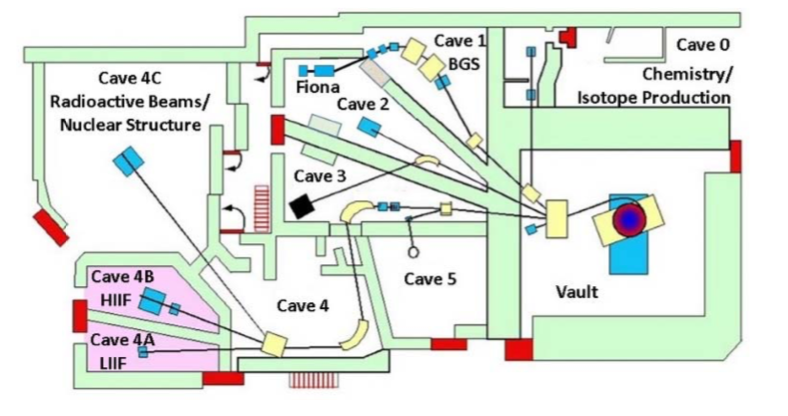
\includegraphics[width=0.5\textwidth]{LBL_88.png}
    \caption{An overview of the facility.  Picture is from \cite{KireeffCovo2018}}
    \label{fig:LBNL_88}
\end{figure}

\subsection{General functionality of a Cyclotron}
Cyclotrons consist of two D-shaped electrodes shaped as a circle with a gap between, and an electromagnet consisting of two coils in which the electrode is placed between. This creates a magnetic field perpendicular to the electrodes. 
From the Lorentz Force, with a magnetic field perpendicular to an electric field will give a circular movement of a particle of charge $q$,

\begin{equation} \label{eq:Lorentz}
    \textbf{F} = q\textbf{E} + q\textbf{v} \times \textbf{B}
\end{equation}

An oscillating electric field is applied between the electrodes, which makes the particles accelerate over the gap between the electrode, be bent in a circular motion and accelerated back with the shifting electrical field. The frequency of the field is called the radio-frequency (RF), or the cyclotron resonance
\begin{equation}
    f = \frac{qB}{2\pi m}
\end{equation}
Particles which are not synchronized with the RF-field is lost \cite{KireeffCovo2018}. \textcolor{red}{Include figure of cyclotron?}  

We can rewrite equation \label{eq:Lorentz}, using the centripetal force, $F_c = \frac{mv^2}{r}$. Since the centripetal force works in the same direction as the magnetic field, we can set $F_c=qvB$, which gives the radius of the particle path 
\begin{equation}
    r = \frac{mv}{qB}
\end{equation}
With increasing velocity, the radius of the path increases. But to obtain the RF, the velocity of the particle must also increase, hence the acceleration over the gap. This way, particles moves in an outward spiral, until they have gained sufficient energy wanted. The cyclotron must be operated in a vacuum, so the beam is not attenuated due to air particles. 


%Description: Describe cross section equation and the different stuff that goes into the equation. Then why we care about the mass density, efficiency. 

\section{The experiment}



The experimental cross section for a nucleus is described in the following equation

\begin{equation} \label{eq:CrossSection_general}
    \sigma(\langle E \rangle) = \frac{A_0}{\rho\Delta r I (1-e^{-\lambda \Delta t})}
\end{equation}



where $\langle E \rangle$ is the average energy across the foil, $A_0$ (Bq) is the activity after end of beam, $\rho \Delta r$ is the areal density of the target (nuclei/cm$^2$), I is the beam current (A), $\lambda$ is the decay constant ($s^{-1}$) of the nucleus and $\Delta t$ (s) is the length of the irradiation. %$A_0$ is found through by backpropagation of activities measured at multiple timepoints after end of beam, and will be further described in section \textcolor{red}{end of beam activity section}. The mass density of an 

Description: Describe cross section equation and the different stuff that goes into the equation. Then why we care about the mass density, efficiency. 



\subsection{Target design}
\textit{\textcolor{red}{Also, write about thin targets, underfilled beam, advantageous.}}\\

\noindent 
In this experiment, a stack of ten thin $^{\text{nat}}$Ir (99.9\%), ten $^{\text{nat}}$Ni, ten $^{\text{nat}}$Cu and three $^{\text{nat}}$Fe foils were irradiated with 33 MeV deuterions to induce nuclear reactions  \textcolor{red}{(provide info about foils, like where they were bought, and abundance and purity of the metal)}. The design of the target stack is well described in the literature (Voyles2018). Using a stacked target in a cross section experiment provides cross sections at multiple energies due to the energy degradation of the beam in the stack. With each foil being approximately 25 $\mu$m in thickness, cross sections were measured within high precision on the energy. Deuterions on Nickel, Cupper and Iron have several well known cross sections, which was used to determine the beam current throughout the stack, by solving equation \ref{eq:CrossSection_general} for beam current, and using these cross sections. These reactions are called monitor reactions, and we were particularly interested in $^{\text{nat}}$Ni(d,x)$^{56,58}$Co, $^{\text{nat}}$Cu(d,x)$^{62, 63, 75}$Zn and $^{\text{nat}}$Fe(d,x)$^{56}$Co.  \\ 

%The targets are larger than the beam, hence underfilled. Then the correct nuc/cmˆ2 
\noindent
In this experiment, the beam was underfilled, meaning that the area of the target was larger than the beamspot. Hence the areal density was then used to calculate the quantity of how many nuclei per cm$^2$. Areal density is given as 
\begin{equation}
    \rho \Delta r = \frac{m}{A}
\end{equation}
\noindent
where m is the mass and A is the area. The uncertainty in each parameter was calculated using the standard deviation 
\begin{equation}
    \sigma = \sqrt{\frac{1}{N}\sum_{i=1}^N (x_i - \overline{x})^2}
\end{equation}
\noindent
where N is the number of measurements, $x_i$ is a measurement and $\overline{x}$ is the average over all measurements. 

\noindent
Since each of these parameters are independent, the uncertainty can be calculated using the approximation for uncertainty 

\begin{equation}
    \Big(\frac{\delta \rho \Delta r}{\rho \Delta r}\Big)^2= \Big(\frac{\delta m}{m}\Big)^2 \Big(\frac{\delta A}{A}\Big)^2
\end{equation}

\noindent 
The foils were cut into approximately 25 by 25 mm squares. Each foil was characterized using a caliper\footnote{MITUTOYO, ABSOLUTE DIGIMATIC} to measure the length of each side, a gauge caliper\footnote{MITUTOYO, IP65 COOLANT PROOF} to measure the thickness, and a weight\footnote{METTLER TOLEDO} was used to weight each foil which were pre-washed with isopropanol. For each foil, the length (across all sides) and thickness was measured at four different locations along the foils (they were not completely uniform). The foils were weighted four times as well. The thickness was not used in the calculation of the mass density, but was a good indication that the foil thicknesses were consistent. Conversion of the areal density to nuclei/$cm^2$ was done numerically, by multiplying by Avogadro's number and dividing by the mol-mass of the target.

\noindent
Table \ref{table:foil_characterization} shows the target stack with average values for length, thickness and areal density, and calculated areal density (in the order they were irradiated). After characterization, each foil was mounted on a plastic frame, and attached with capton tape along the edges. The target frames can be seen in figure \ref{fig:targetframe}. 


\begin{table}[h!]
%\centering
\caption{Characterization of each foil, along with calculated mass density. Each length is measured in mm, and mass in grams. }
\label{table:foil_characterization}
\small
\begin{tabular}{lllllll}
\makecell{\textbf{Foil}} & \makecell{Length1 (mm)}  &  \makecell{Length2 (mm)} & \makecell{Thickness (mm)} & \makecell{Mass (g)} & \makecell{\textbf{Mass density (mg/cm$^2$)}} \\ 
\hline
\makecell{SS1} & \makecell{} & \makecell{} & \makecell{} & \makecell{} & \makecell{\textbf{...}} \\
\hline
\makecell{Ni01} & \makecell{25.228} & \makecell{25.293} & \makecell{0.0285} & \makecell{0.1453} & \makecell{22.772 $\pm$ 0.138} \\
\makecell{Ir01} & \makecell{24.943} & \makecell{24.968} & \makecell{0.0295} & \makecell{0.3436} & \makecell{55.174 $\pm$ 0.053} \\
\makecell{Cu01} & \makecell{25.553} & \makecell{24.883} & \makecell{0.0341} & \makecell{0.1420} & \makecell{22.338 $\pm$ 0.048} \\
\makecell{Fe01} & \makecell{24.400} & \makecell{26.068} & \makecell{0.0278} & \makecell{0.1274} & \makecell{20.030 $\pm$ 0.110} \\
\hline
\makecell{Ni02} & \makecell{25.288} & \makecell{25.428} & \makecell{0.0295} & \makecell{0.1487} & \makecell{23.118 $\pm$ 0.096} \\
\makecell{Ir02} & \makecell{24.923} & \makecell{25.005} & \makecell{0.0278} & \makecell{0.3465} & \makecell{55.601 $\pm$ 0.238} \\
\makecell{Cu02} & \makecell{25.443} & \makecell{25.550} & \makecell{0.0348} & \makecell{0.1451} & \makecell{22.325 $\pm$ 0.028} \\
\makecell{Fe02} & \makecell{25.525} & \makecell{23.800} & \makecell{0.0274} & \makecell{0.1216} & \makecell{20.017 $\pm$ 0.034} \\
\hline
\makecell{Ni03} & \makecell{25.295} & \makecell{25.210} & \makecell{0.0270} & \makecell{0.1425} & \makecell{22.338 $\pm$ 0.066} \\
\makecell{Ir03} & \makecell{24.885} & \makecell{24.983} & \makecell{0.0243} & \makecell{0.3459} & \makecell{55.643 $\pm$ 0.121} \\
\makecell{Cu03} & \makecell{25.560} & \makecell{25.508} & \makecell{0.0343} & \makecell{0.1455} & \makecell{22.313 $\pm$ 0.043} \\
\makecell{Fe03} & \makecell{26.113} & \makecell{25.235} & \makecell{0.0310} & \makecell{0.1315} & \makecell{19.948 $\pm$ 0.114} \\
\hline
\makecell{Ni04} & \makecell{25.303} & \makecell{24.888} & \makecell{0.0273} & \makecell{0.1304} & \makecell{20.704 $\pm$ 0.068} \\
\makecell{Ir04} & \makecell{24.960} & \makecell{24.833} & \makecell{0.0261} & \makecell{0.3471} & \makecell{56.000 $\pm$ 0.109} \\
\makecell{Cu04} & \makecell{25.153} & \makecell{25.603} & \makecell{0.0333} & \makecell{0.1435} & \makecell{22.284 $\pm$ 0.027} \\
\hline
\makecell{Ni05} & \makecell{25.325} & \makecell{25.495} & \makecell{0.0263} & \makecell{0.1406} & \makecell{21.768 $\pm$ 0.045} \\
\makecell{Ir05} & \makecell{24.948} & \makecell{24.958} & \makecell{0.0256} & \makecell{0.3435} & \makecell{55.161 $\pm$ 0.081} \\
\makecell{Cu05} & \makecell{25.213} & \makecell{25.573} & \makecell{0.0334} & \makecell{0.1447} & \makecell{22.443 $\pm$ 0.028} \\
\hline
\makecell{Ni06} & \makecell{25.530} & \makecell{25.195} & \makecell{0.0285} & \makecell{0.1471} & \makecell{22.861 $\pm$ 0.123} \\
\makecell{Ir06} & \makecell{24.760} & \makecell{24.960} & 
\makecell{0.0240} & \makecell{0.3444} & \makecell{55.731 $\pm$ 0.088} \\
\makecell{Cu06} & \makecell{25.343} & \makecell{25.513} & \makecell{0.0340} & \makecell{0.1448} & \makecell{22.396 $\pm$ 0.012} \\
\hline
\makecell{Ni07} & \makecell{25.338} & \makecell{25.278} & \makecell{0.0268} & \makecell{0.1479} & \makecell{23.092 $\pm$ 0.078} \\
\makecell{Ir07} & \makecell{24.955} & \makecell{25.008} & \makecell{0.0278} & \makecell{0.3538} & \makecell{56.685 $\pm$ 0.085} \\
\makecell{Cu07} & \makecell{25.625} & \makecell{25.248} & \makecell{0.0326} & \makecell{0.1444} & \makecell{22.320 $\pm$ 0.014} \\
\hline
\makecell{Ni08} & \makecell{25.205} & \makecell{24.950} & \makecell{0.0256} & \makecell{0.1409} & \makecell{22.409 $\pm$ 0.124} \\
\makecell{Ir08} & \makecell{24.723} & \makecell{24.985} & \makecell{0.0281} & \makecell{0.3585} & \makecell{58.030 $\pm$ 0.130} \\
\makecell{Cu08} & \makecell{25.370} & \makecell{24.885} & \makecell{0.0333} & \makecell{0.1414} & \makecell{22.401 $\pm$ 0.033} \\
\hline
\makecell{Ni09} & \makecell{25.220} & \makecell{25.378} & \makecell{0.0257} & \makecell{0.1392} & \makecell{21.741 $\pm$ 0.073} \\
\makecell{Ir09} & \makecell{24.670} & \makecell{24.993} & \makecell{0.0273} & \makecell{0.3494} & \makecell{56.669 $\pm$ 0.043} \\
\makecell{Cu09} & \makecell{25.390} & \makecell{26.455} & \makecell{0.0331} & \makecell{0.1506} & \makecell{22.425 $\pm$ 0.041} \\
\hline
\makecell{Ni10} & \makecell{25.285} & \makecell{24.405} & \makecell{0.0271} & \makecell{0.1425} & \makecell{23.093 $\pm$ 0.024} \\
\makecell{Ir10} & \makecell{24.973} & \makecell{24.980} & \makecell{0.0270} & \makecell{0.3435} & \makecell{55.065 $\pm$ 0.055} \\
\makecell{Cu10} & \makecell{25.470} & \makecell{25.338} & \makecell{0.0355} & \makecell{0.1440} & \makecell{22.314 $\pm$ 0.047} \\
\hline


\hline
\makecell{SS2} & \makecell{} & \makecell{} & \makecell{} & \makecell{} & \makecell{\textbf{...}} \\
\makecell{P-degrader} & \makecell{} & \makecell{} & \makecell{} & \makecell{} & \makecell{\textbf{...}} \\
\makecell{Ni neutron monitor} & \makecell{} & \makecell{} & \makecell{} & \makecell{} & \makecell{\textbf{...}} \\
\hline
\end{tabular}
\end{table}

\begin{figure}
    \centering
    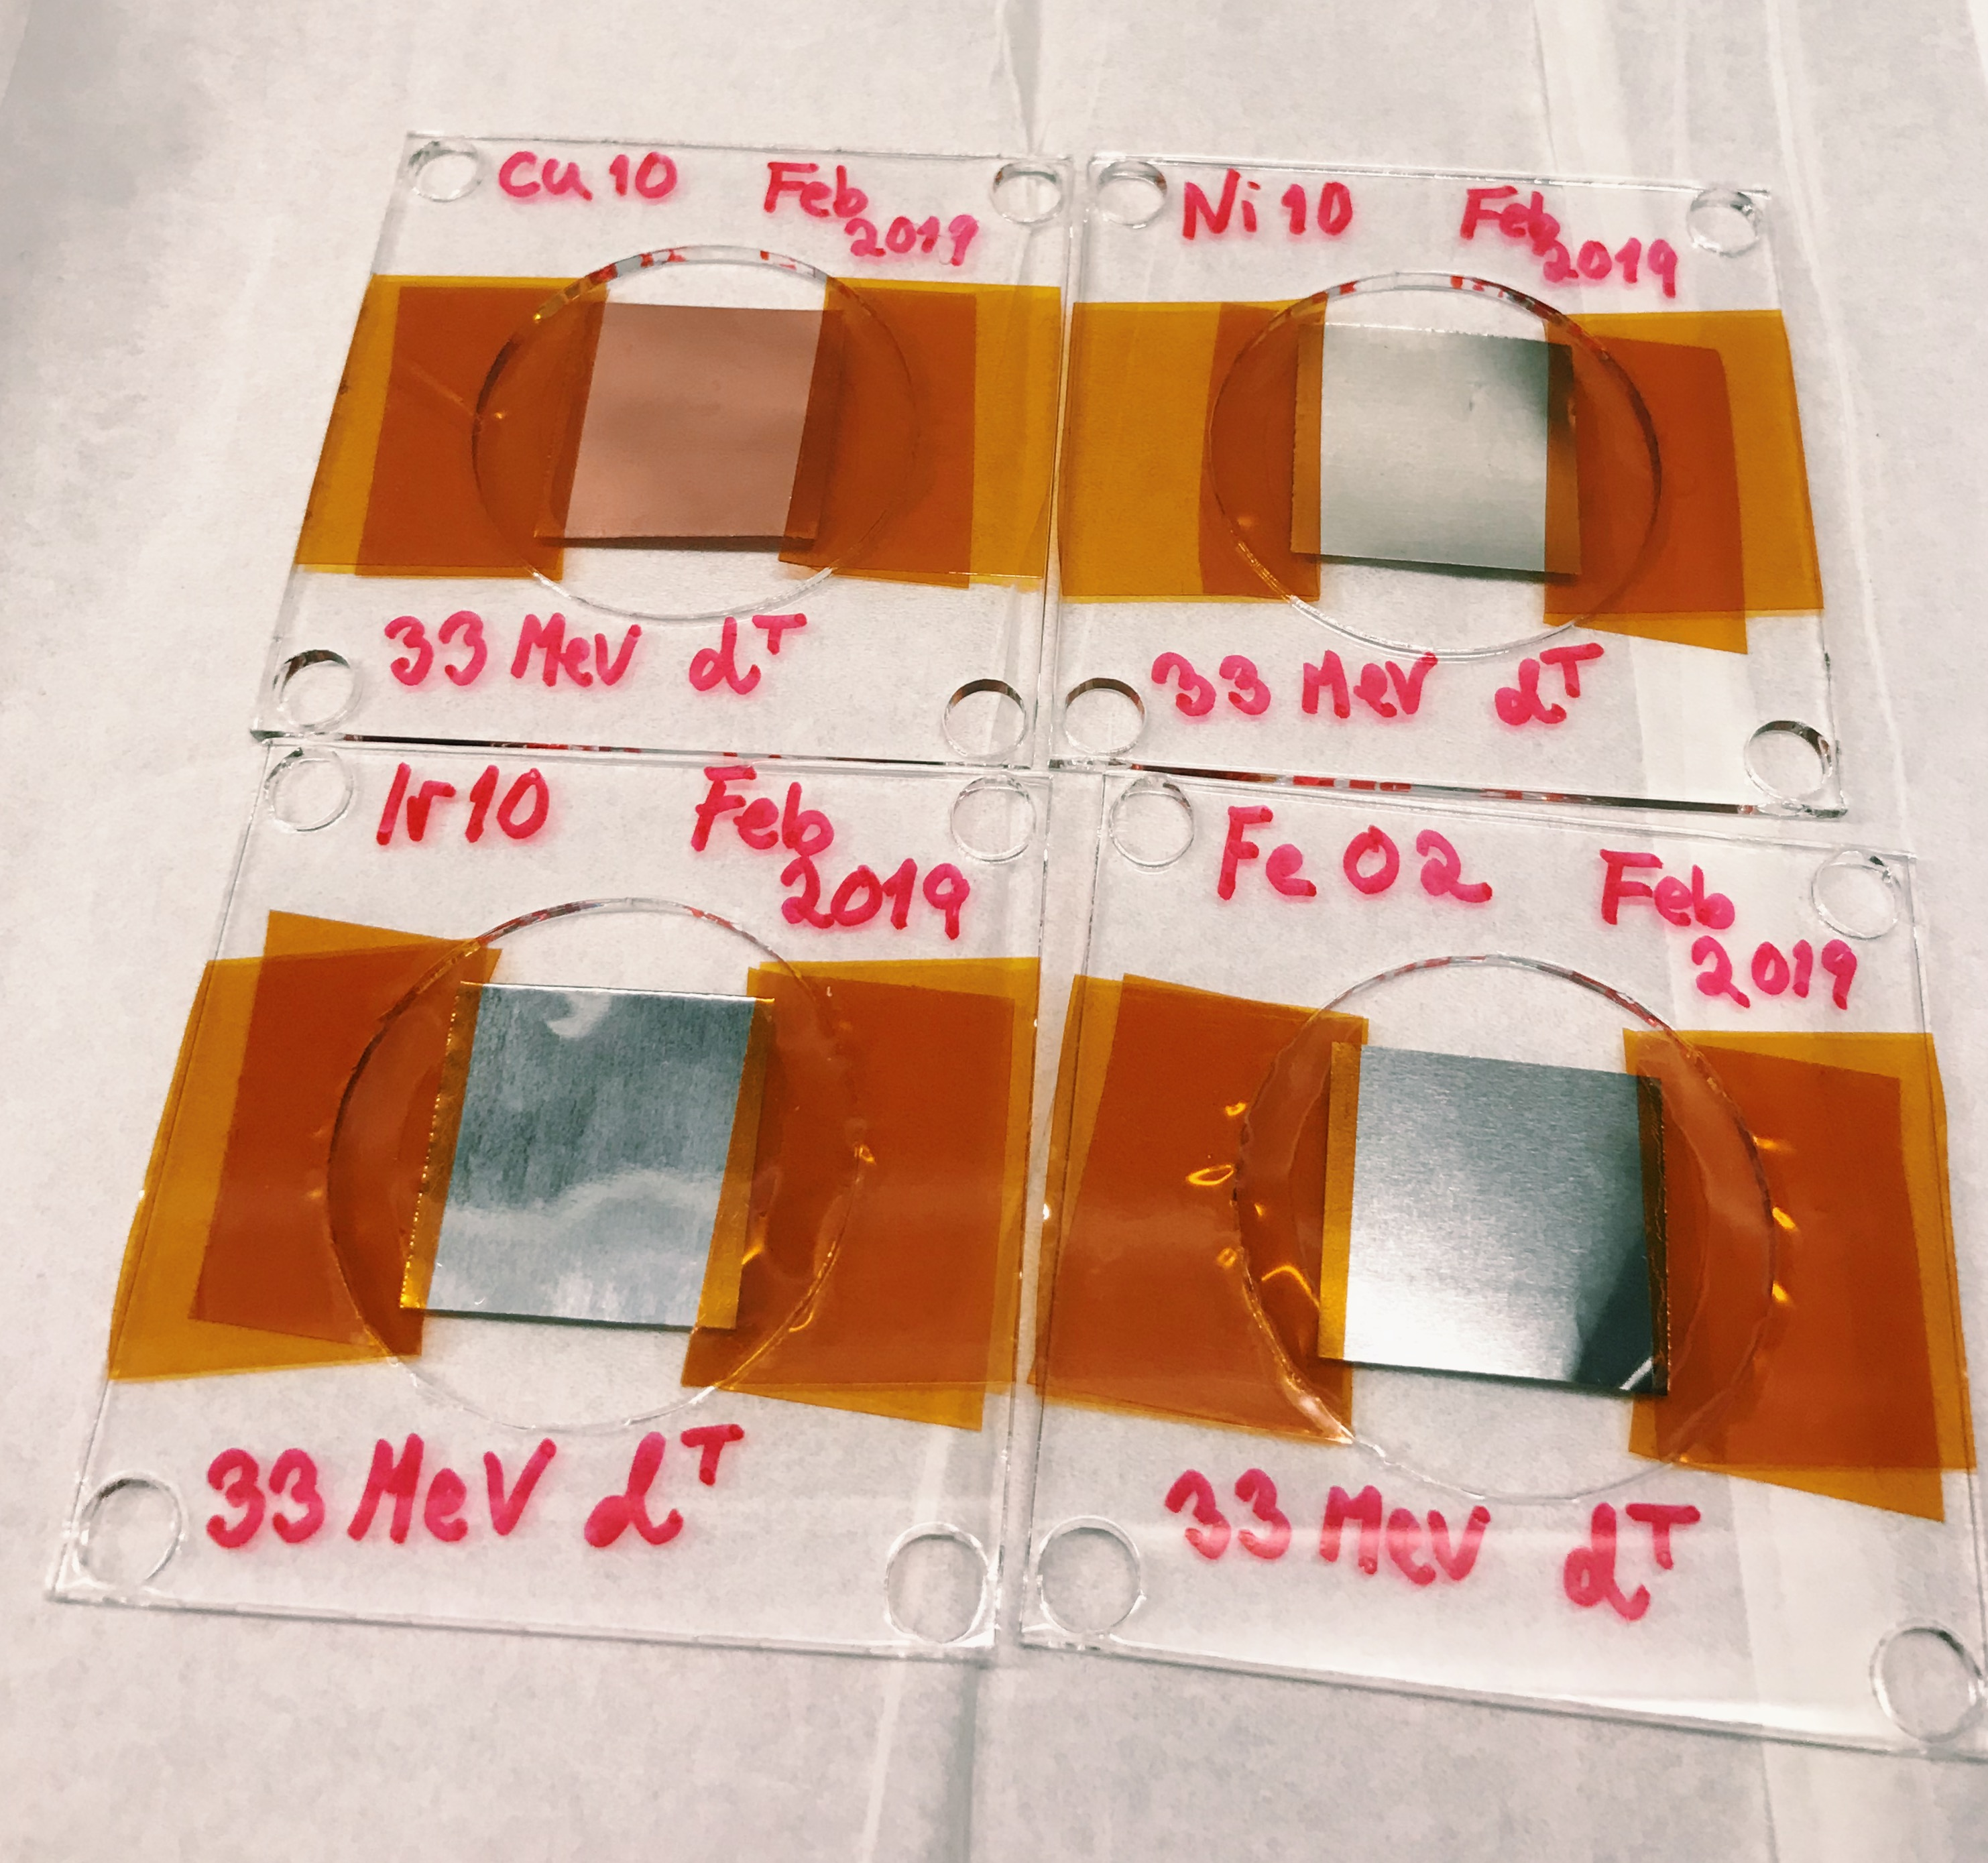
\includegraphics[width=8cm]{targetframe.JPG}
    
    \caption{The target foils were mounted on plastic frames using capton tape. }
    \label{fig:targetframe}
\end{figure}

\subsection{Detector calibration}
In this experiment, seven different high purity Germanium detectors (HPGe) were used to measure the activity in each foil at multiple timepoints after end of beam. The HPGe-detector is a type of semiconductor, which is a material where the energy required to remove an electron from the valence band (in the outer atomic shell) to the conduction band is small. A Germanium atom has atomic number 32, and 4 valence electrons in the outer p4 shell. The atoms are bound through covalent bonds in a crystal structure. The main mechanism of a semiconductor detector is creation of electron-hole pairs after energy deposition of an ionizing particle in the crystal. If an electron is excited to the conduction band, a hole is left. The hole can move as a neighbooring electron fills this spot, and it can cause a chain reaction, and the hole will move in the crystal. Both the electron in the conduction band and the hole in  the valence band contributes to an electric current. Under influence of an electric field, the electron-hole pairs will be collected, and we can measure the incidence as a count. The major advantage with semiconductor detector is that the average energy to create an electron-hole pair is very low, which results in a superior energy resolution in comparison to other detectors like gas and scintillation detectors. \textcolor{red}{High energy resolution advantageous in gamma-ray spectroscopy which makes it possible to separate to gamma-ray peaks within less than a keV.} At room temperature,  thermal energy can excite the electron from the valence to the conduction band and cause noise in spectra. Therefor, Germanium detectors are operated at 0 Kelvin. \textcolor{red}{Write about recombination and trapping, noise, np semiconductor junction, depletion depth??}. (Techniques for Nuclear and Particle Physics Experiments. William R. Leo. Second Revised Edition. Springer.Verlag Berkling Heidelberg GmbH, New York (1994). p. 215-216 )\\


\noindent
\textcolor{red}{
The detectors along with crystal geometry and dimension is listed in table \ref{tab:detector_characteristics}. Detector 1-6 was counted in cave 4c, which is an old beam chamber. Hence, background radiation from ........ are present in the room. Detector 7 was counted in a room with little backgrond, and also led shielding surronding the detector. }


\subsubsection{Detector efficiency}
The detector efficiency is the number of events registered divided by the events emitted by the source. The absolute efficiency can be divided into intrinsic and geometrical efficiency, where the intrinsic efficiency is the number of evens registered divided by the number of evens hitting the detector. The intrinsic efficiency thus depends on the interaction cross section between incident particle and detector material. For neutral particles, the size of the detector affects the intrinsic efficiency, the larger crystal the larger the probability of interaction is. The geometrical efficiency is the radiation emitted by the source which hits the detector. (Techniques for Nuclear and Particle Physics Experiments. William R. Leo. Second Revised Edition. Springer.Verlag Berkling Heidelberg GmbH, New York (1994). p. 121-122 )\\ 




\noindent 
In calculation of the efficiency of each detector, calibration point sources $^{137}$Cs ($t_{1/2}$=30.08 years), $^{133}$Ba ($t_{1/2}$=10.551 years) and $^{152}$Eu ($t_{1/2}$=13.517 years) was used. Figure \ref{fig:cal_sources} shows the sources along with activity at reference date which was January 1$^{\text{st}}$, 2009. \textcolor{red}{ $^{22}$Na was initially planned to be used, however was excluded due to difficulties with the gamma line}. Table \ref{table:calibration_gammas} shows an overview of the different gamma lines that was used in order to calculate the efficiency. The calibration sources were counted on all the different detectors at specific distances from the detector. Maestro\footnote{https://www.ortec-online.com/products/application-software/maestro-mca} (Multichannel Analyzer Emulation Software) was used in spectroscopy.  \\

\noindent 
\textcolor{red}{
A detector has a dead layer, and the radiation needs sufficient energy to penetrate through this window. }


\begin{figure}
    \centering
    \includegraphics[width=8cm]{cal_sources.png}
    \caption{Calibration sources that were used in the calibration of the detectors.}
    \label{fig:cal_sources}
\end{figure}

\noindent 
The activity of the calibration sources at the time between the reference date and the date measurement (referred to as delay time) is 
\begin{equation}
    A(t) = A_0 e^{-\lambda \Delta t_\text{delay}}
\end{equation}
\noindent
where $A_0$ is the activity on the reference date and $\lambda$ is the decay constant. The total number of decayed nuclei since the reference date and during the count is 
\begin{equation}
\Delta D = -\int_{\Delta t_\text{delay}}^{\Delta t_\text{delay}+\Delta t_\text{livetime}} A(t)dt
\end{equation}
\noindent 
Solving the integral, the number of decayed nuclei since the reference date is 
\begin{equation}
    \Delta D = \frac{A_0}{\lambda}e^{-\lambda \Delta t_\text{delay}}(1-e^{-\lambda \Delta t_\text{live}})
\end{equation}

\noindent
where the live is the livetime of the spectrum is the time it was counting events \textcolor{red}{(the real time which has accounted for the deadtime, the time where the system is enable to register events after an event)}. 
The net area of the peak is described as 
\begin{equation}
    N_C = \Delta D I_\gamma \epsilon(E_\gamma)
\end{equation} 

\noindent 
which gives us an efficiency as a function of $E_\gamma$

\begin{equation} \label{eq:efficiency}
    \epsilon(E_\gamma)=\frac{\lambda N_C}{A_0 I_\gamma(1-e^{-\lambda \Delta t_\text{live}})e^{-\lambda \Delta t_\text{delay}}}
\end{equation}

\noindent
Equation \ref{eq:efficiency} gives the efficiency value at one specific $E_\gamma$. In order to find a general efficiency curve for the detector, a model based upon  Gallagher, W.J., & Cipolla, S.J. (1974) was applied, which takes the probability of penetration through the deadlayer of the detector and the probability of interaction in detector volume into account: 

\begin{equation} \label{eq:efficiency_estimated}
\epsilon(E_\gamma) =  B_0 + \underbrace{(e^{-B_1 E_\gamma^{B_2}})}_\text{dead layer}  \underbrace{(1-e^{-B_3 E_\gamma^{B_4}}))}_\text{interacting with volume} 
\end{equation}
\noindent
where $B_0$, $B_1$, $B_2$, $B_3$ and $B_4$ are guessing parameters which were found through the scipy curve fit function\footnote{\url{https://docs.scipy.org/doc/scipy/reference/generated/scipy.optimize.curve_fit.html}}. An example of an efficiency curve can be seen in figure \ref{fig:efficiency_curve}.  %Figure \ref{fig:ex_eff_curve} shows an example for such a fitted efficiency curve. When guessing parameters are found, we have efficiency for the detector at any gamma energy.

\begin{figure}
    \centering
    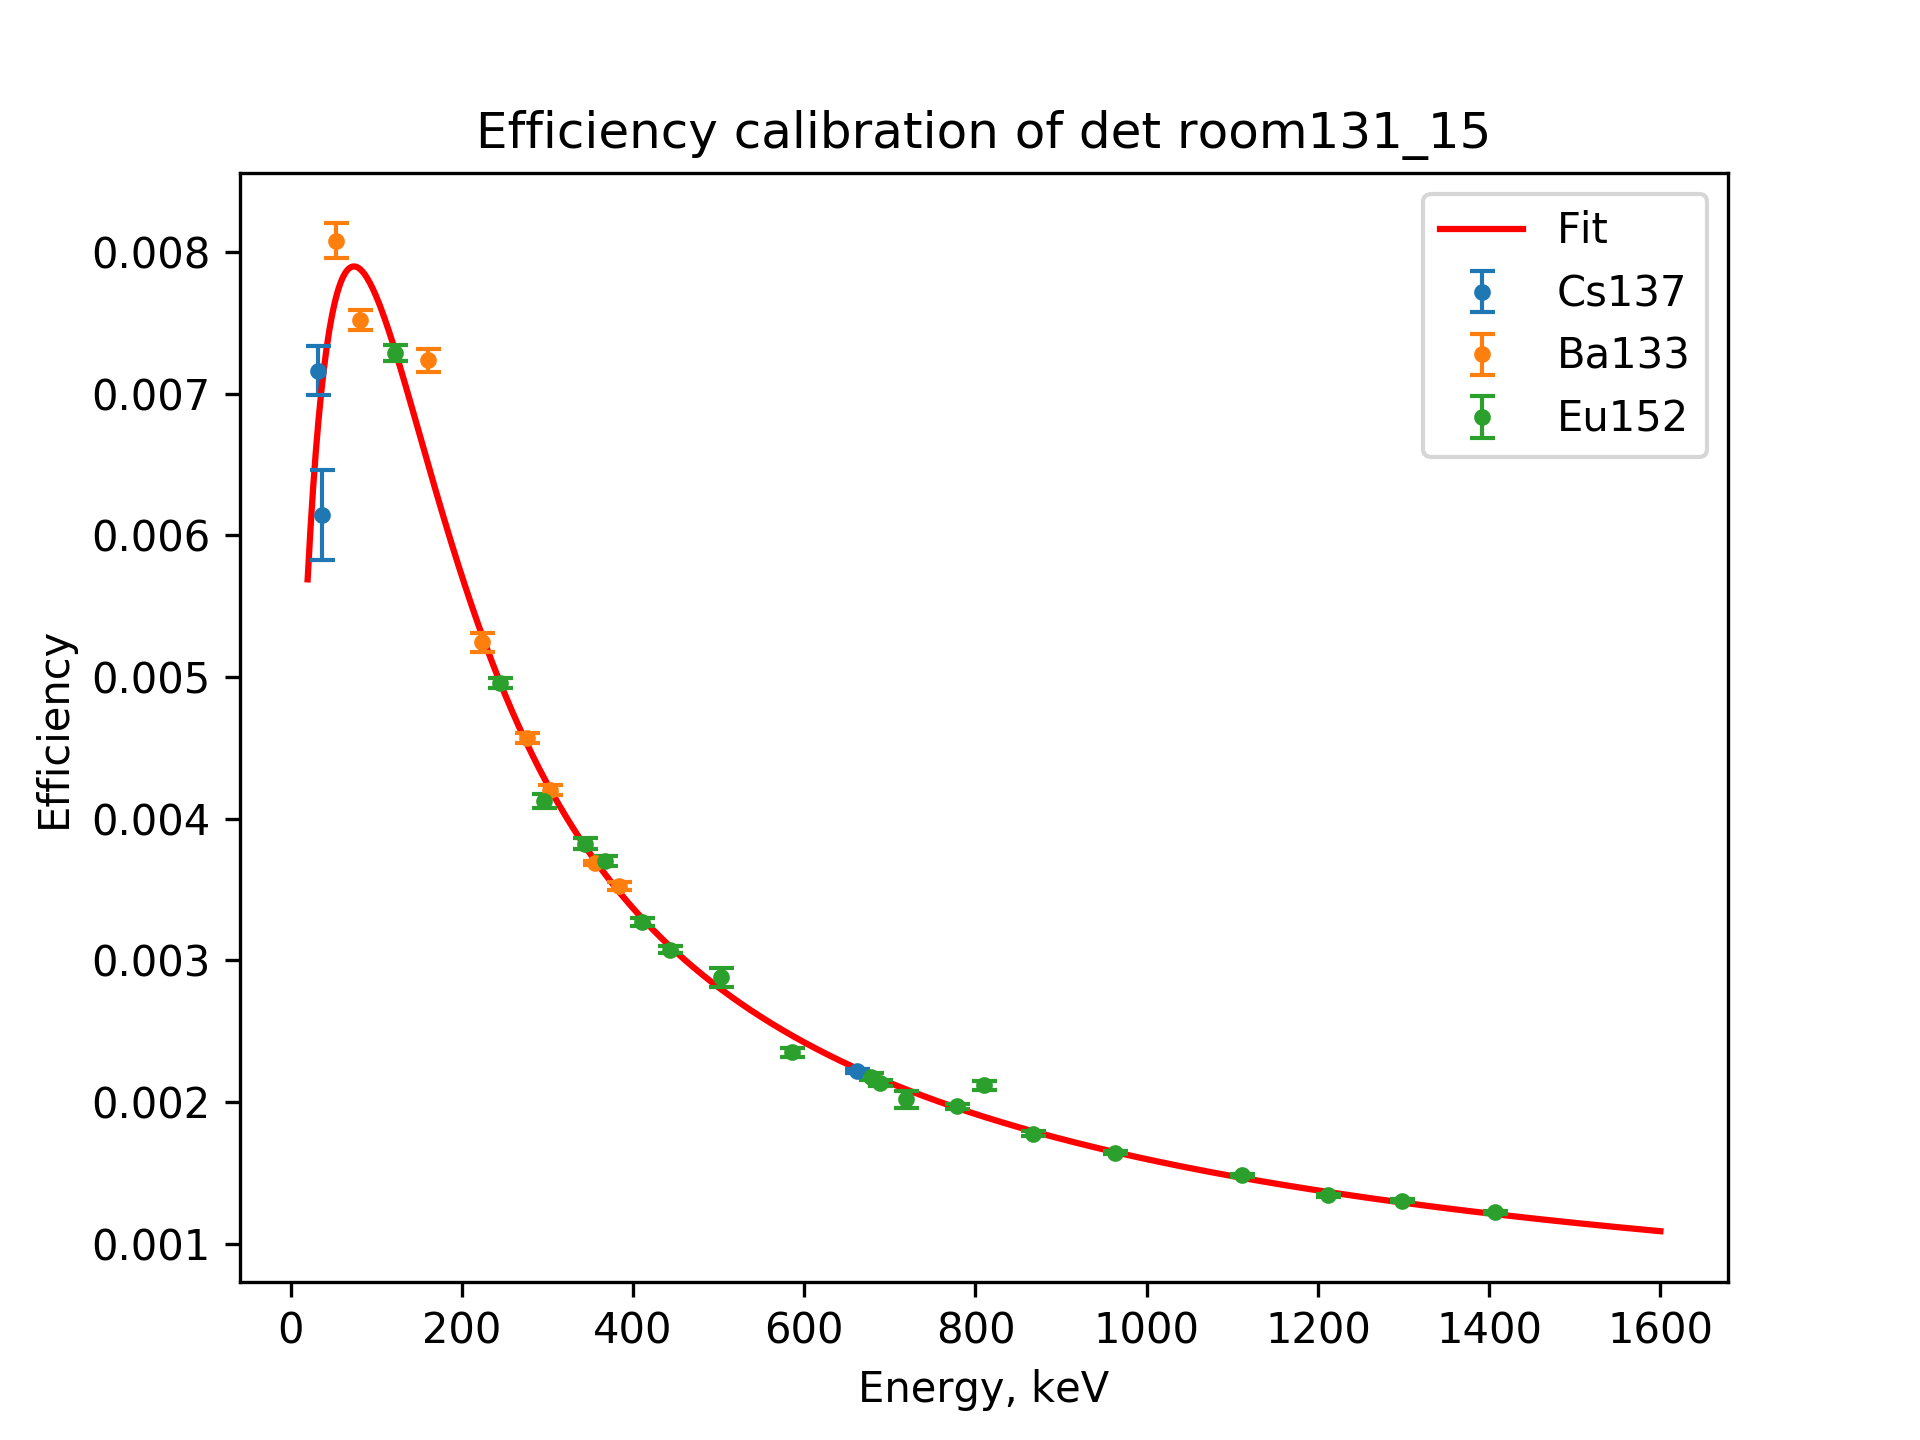
\includegraphics[width=8cm]{room131_15.png}
    \caption{An example of an efficiency curve}
    \label{fig:efficiency_curve}
\end{figure}


\begin{table}[]
    \centering
    \caption{The calibration point sources along with gamma lines used. * indicates that the value has been averaged over two peaks with similar energy. For the intensity its just added together. }
    \begin{tabular}{|cc|cc|cc|}
        \hline
        
         \multicolumn{2}{|c}{\makecell{^{137}Cs}} & \multicolumn{2}{c}{\makecell{^{133}Ba}} & \multicolumn{2}{c|}{\makecell{^{152}Eu}}\\
         %\hline 
         \Xhline{2\arrayrulewidth}
         \makecell{E_\gamma}& \makecell{I_\gamma}&\makecell{E_\gamma}& \makecell{I_\gamma}& \makecell{E_\gamma}& \makecell{I_\gamma}\\
         \hline
         \makecell{32.005^*} & \makecell{5.63\%^*} & \makecell{53.1622} & \makecell{2.14\%} & \makecell{121.7817} & \makecell{28.53\%}\\
         
         \makecell{36.3405^*} & \makecell{1.02\%^*} & \makecell{80.9979} & \makecell{32.9\%} & \makecell{244.6979} & \makecell{7.55\%}\\
         
         \makecell{661.657} & \makecell{85.10\%} & \makecell{160.6120} & \makecell{0.638\%} & \makecell{295.9387} & \makecell{0.440\%}\\
         
          &  & \makecell{223.2368} & \makecell{0.453\%} & \makecell{344.2785} & \makecell{26.5\%}\\
         
          &  & \makecell{276.3989} & \makecell{7.16\%} & \makecell{367.7891} & \makecell{0.859\%}\\
         
          &  & \makecell{302.8508} & \makecell{18.34\%} & \makecell{411.1165} & \makecell{2.237\%}\\
          
          
          & \textcolor{red}{FINISH IF INCLUDING} & \makecell{302.8508} & \makecell{18.34\%} & \makecell{411.1165} & \makecell{2.237\%}\\
  
        %\makecell{^{137}Cs} & \makecell{^{133}Ba} & \makecell{^{152}Eu} \\
        \hline 
   
        \hline
    \end{tabular}
    \label{table:calibration_gammas}
\end{table}

\begin{table}[]
    \centering
    \caption{Table shows the geometry of the different detectors. }
    \begin{tabular}{|c|c|c|}
        \hline\textbf{}
        Detector & Geometry & Dimension \\
        \hline 
        \makecell{Detector 1} & \makecell{..} & \makecell{..} \\
        \makecell{Detector 1} & \makecell{..} & \makecell{..} \\      
        \makecell{Detector 3} & \makecell{..} & \makecell{..} \\     
        \makecell{Detector 4} & \makecell{..} & \makecell{..} \\  
        \makecell{Detector 5} & \makecell{..} & \makecell{..} \\    
        \makecell{Detector 6} & \makecell{..} & \makecell{..} \\      
        \makecell{Detector 7} & \makecell{..} & \makecell{..} \\     
        \hline
    \end{tabular}
    \label{tab:detector_characteristics}
\end{table}


\noindent 
\subsubsection{Energy and peakshape calibration}
Each spectra that was taken was analyzed using FitzPeakz\footnote{https://www.jimfitz.co.uk/fitzpeak.htm}. \textcolor{red}{Write about how the program identifies peaks (read the article). The main mechanism  to search for peaks.  Explain how the detectors were calibrated using energy and peak shape. Each detector was calibrated using a..... }


\subsection{Irradiaton of target stack}
The irradiation of the target stack included a tuning of the beam and one hour of irradiation. Before we could turn on beam, we had to pump down the tube to a vacuum, to not attenuate the beam. \textcolor{red}{check the vacuum in notes}


\subsection{Tuning of the beam}
Before irradiation, the beam was tuned to have the \textcolor{red}{correct energy and beam spot}. The first step was to visualize the beam spot. \textcolor{red}{A glass plate with a 1 cm cross in the center that was painted with phosphorus was placed in the end of the beam tube}. With a camera placed in Cave 0 (not in the beamline), we could visualize the beamspot in the control room. This way, it was possible to steer the beam to be perfectly centered, which was important for the following experiment which used small targets. The next step was to visualize the beam over the target stack, \textcolor{red}{to make sure that the beam did not converge/diverge, spread?}. Gafchromic film changes color when exposed to ionizing radiation. A film was placed in the front and in the back of the target holder, and exposed for a brief seconds. This was done a couple of times before we were satisfied with the beamspot. \\

\noindent 
The last part of the beam tuning was to find beam efficiency of transmission which was done measuring the current at the Faraday cup right after the cyclotron vaul (BS-2) and right before cave 0 (FC-01). BS-2 was measured to be 420 nA, and FC-01 was measured to be 285 nA. This gave a beam efficiency of transmission
\begin{equation*}
    \frac{FC-01}{BS-02}=67\%
\end{equation*}
\noindent 
\textcolor{red}{In reference, .... Se over notater en gang til!}
\begin{comment}
Faraday cup right after Cyclotron vault $$BS-2 = 420 nA$$, and right before cave 0 was $$FC-01=285 nA$$

That gives a beam efficiency of transmission 

$$\frac{FC-01}{BS-02}=67.9\%$$
\end{comment}
\subsection{The irradiation of the target stack}

Figure \ref{fig:stack} shows the targets stacked in the beam holder, and figure \ref{fig:tube} shows how it was placed in the beam tube. 

\begin{figure}
    \centering
    \begin{subfigure}[b]{0.3\textwidth}
        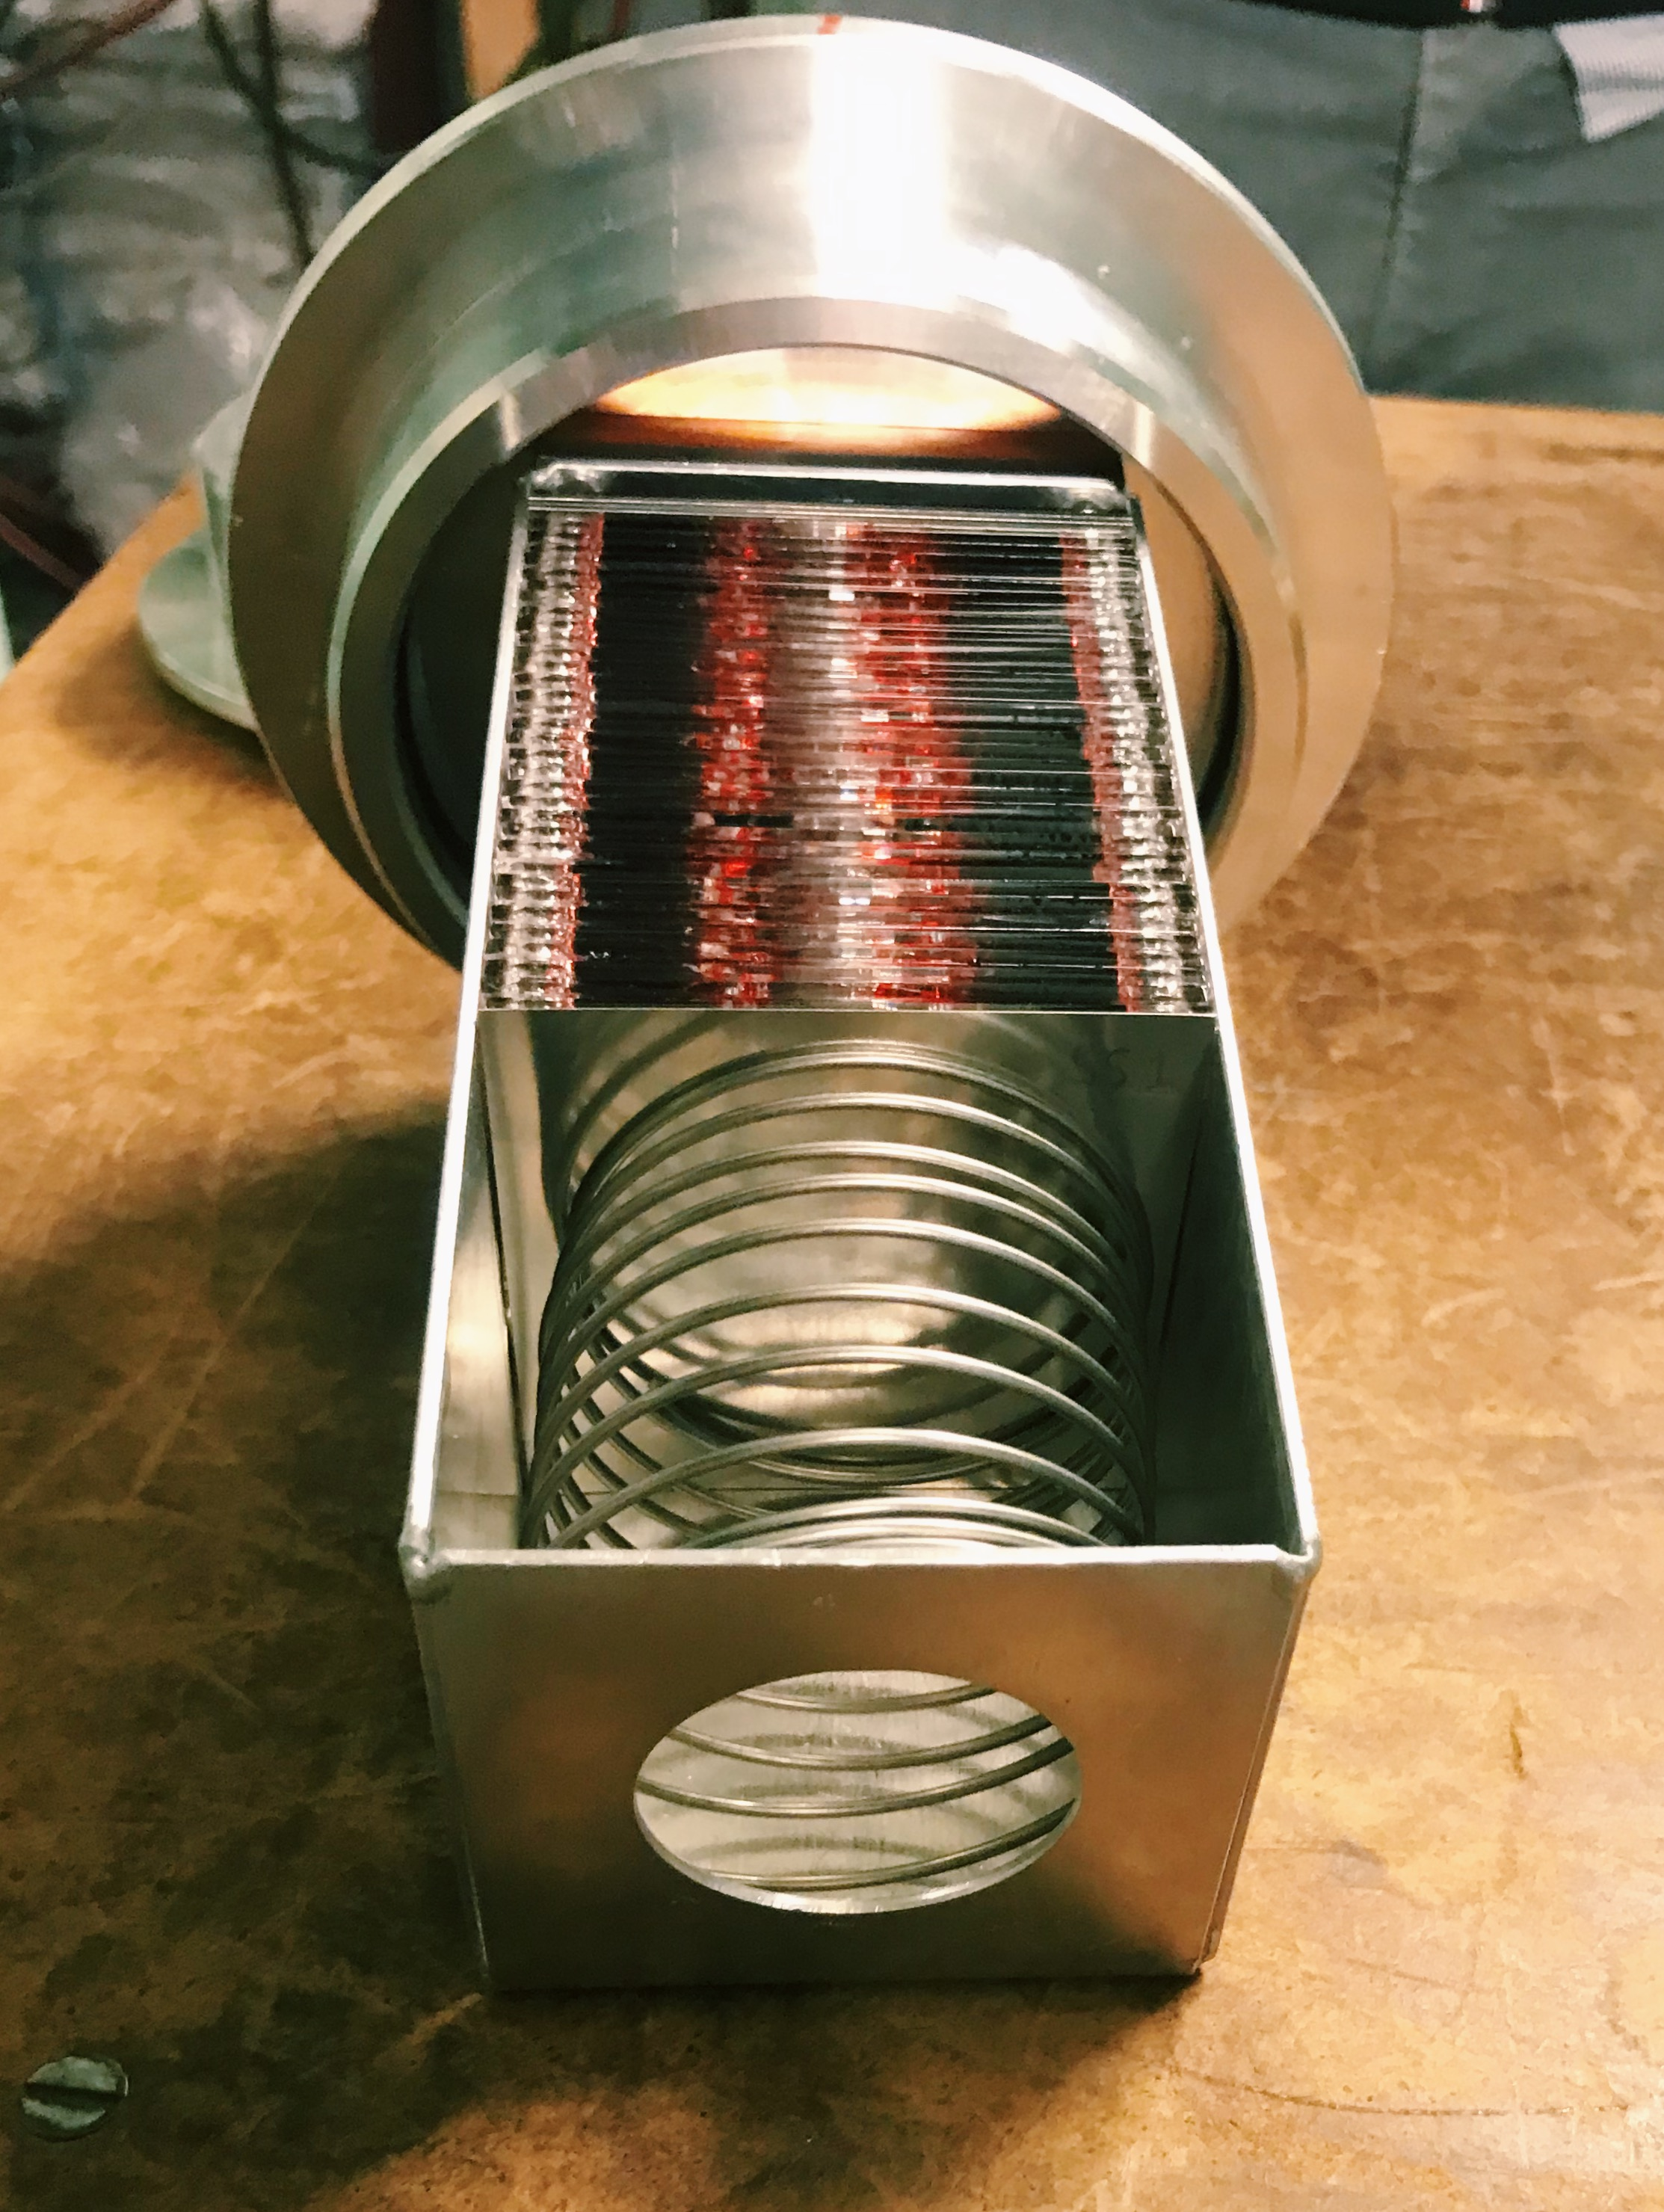
\includegraphics[width=\textwidth]{stack.JPG}
        \caption{Foil stack}
        \label{fig:stack}
    \end{subfigure}
    ~ %add desired spacing between images, e. g. ~, \quad, \qquad, \hfill etc. 
      %(or a blank line to force the subfigure onto a new line)
    \begin{subfigure}[b]{0.3\textwidth}
        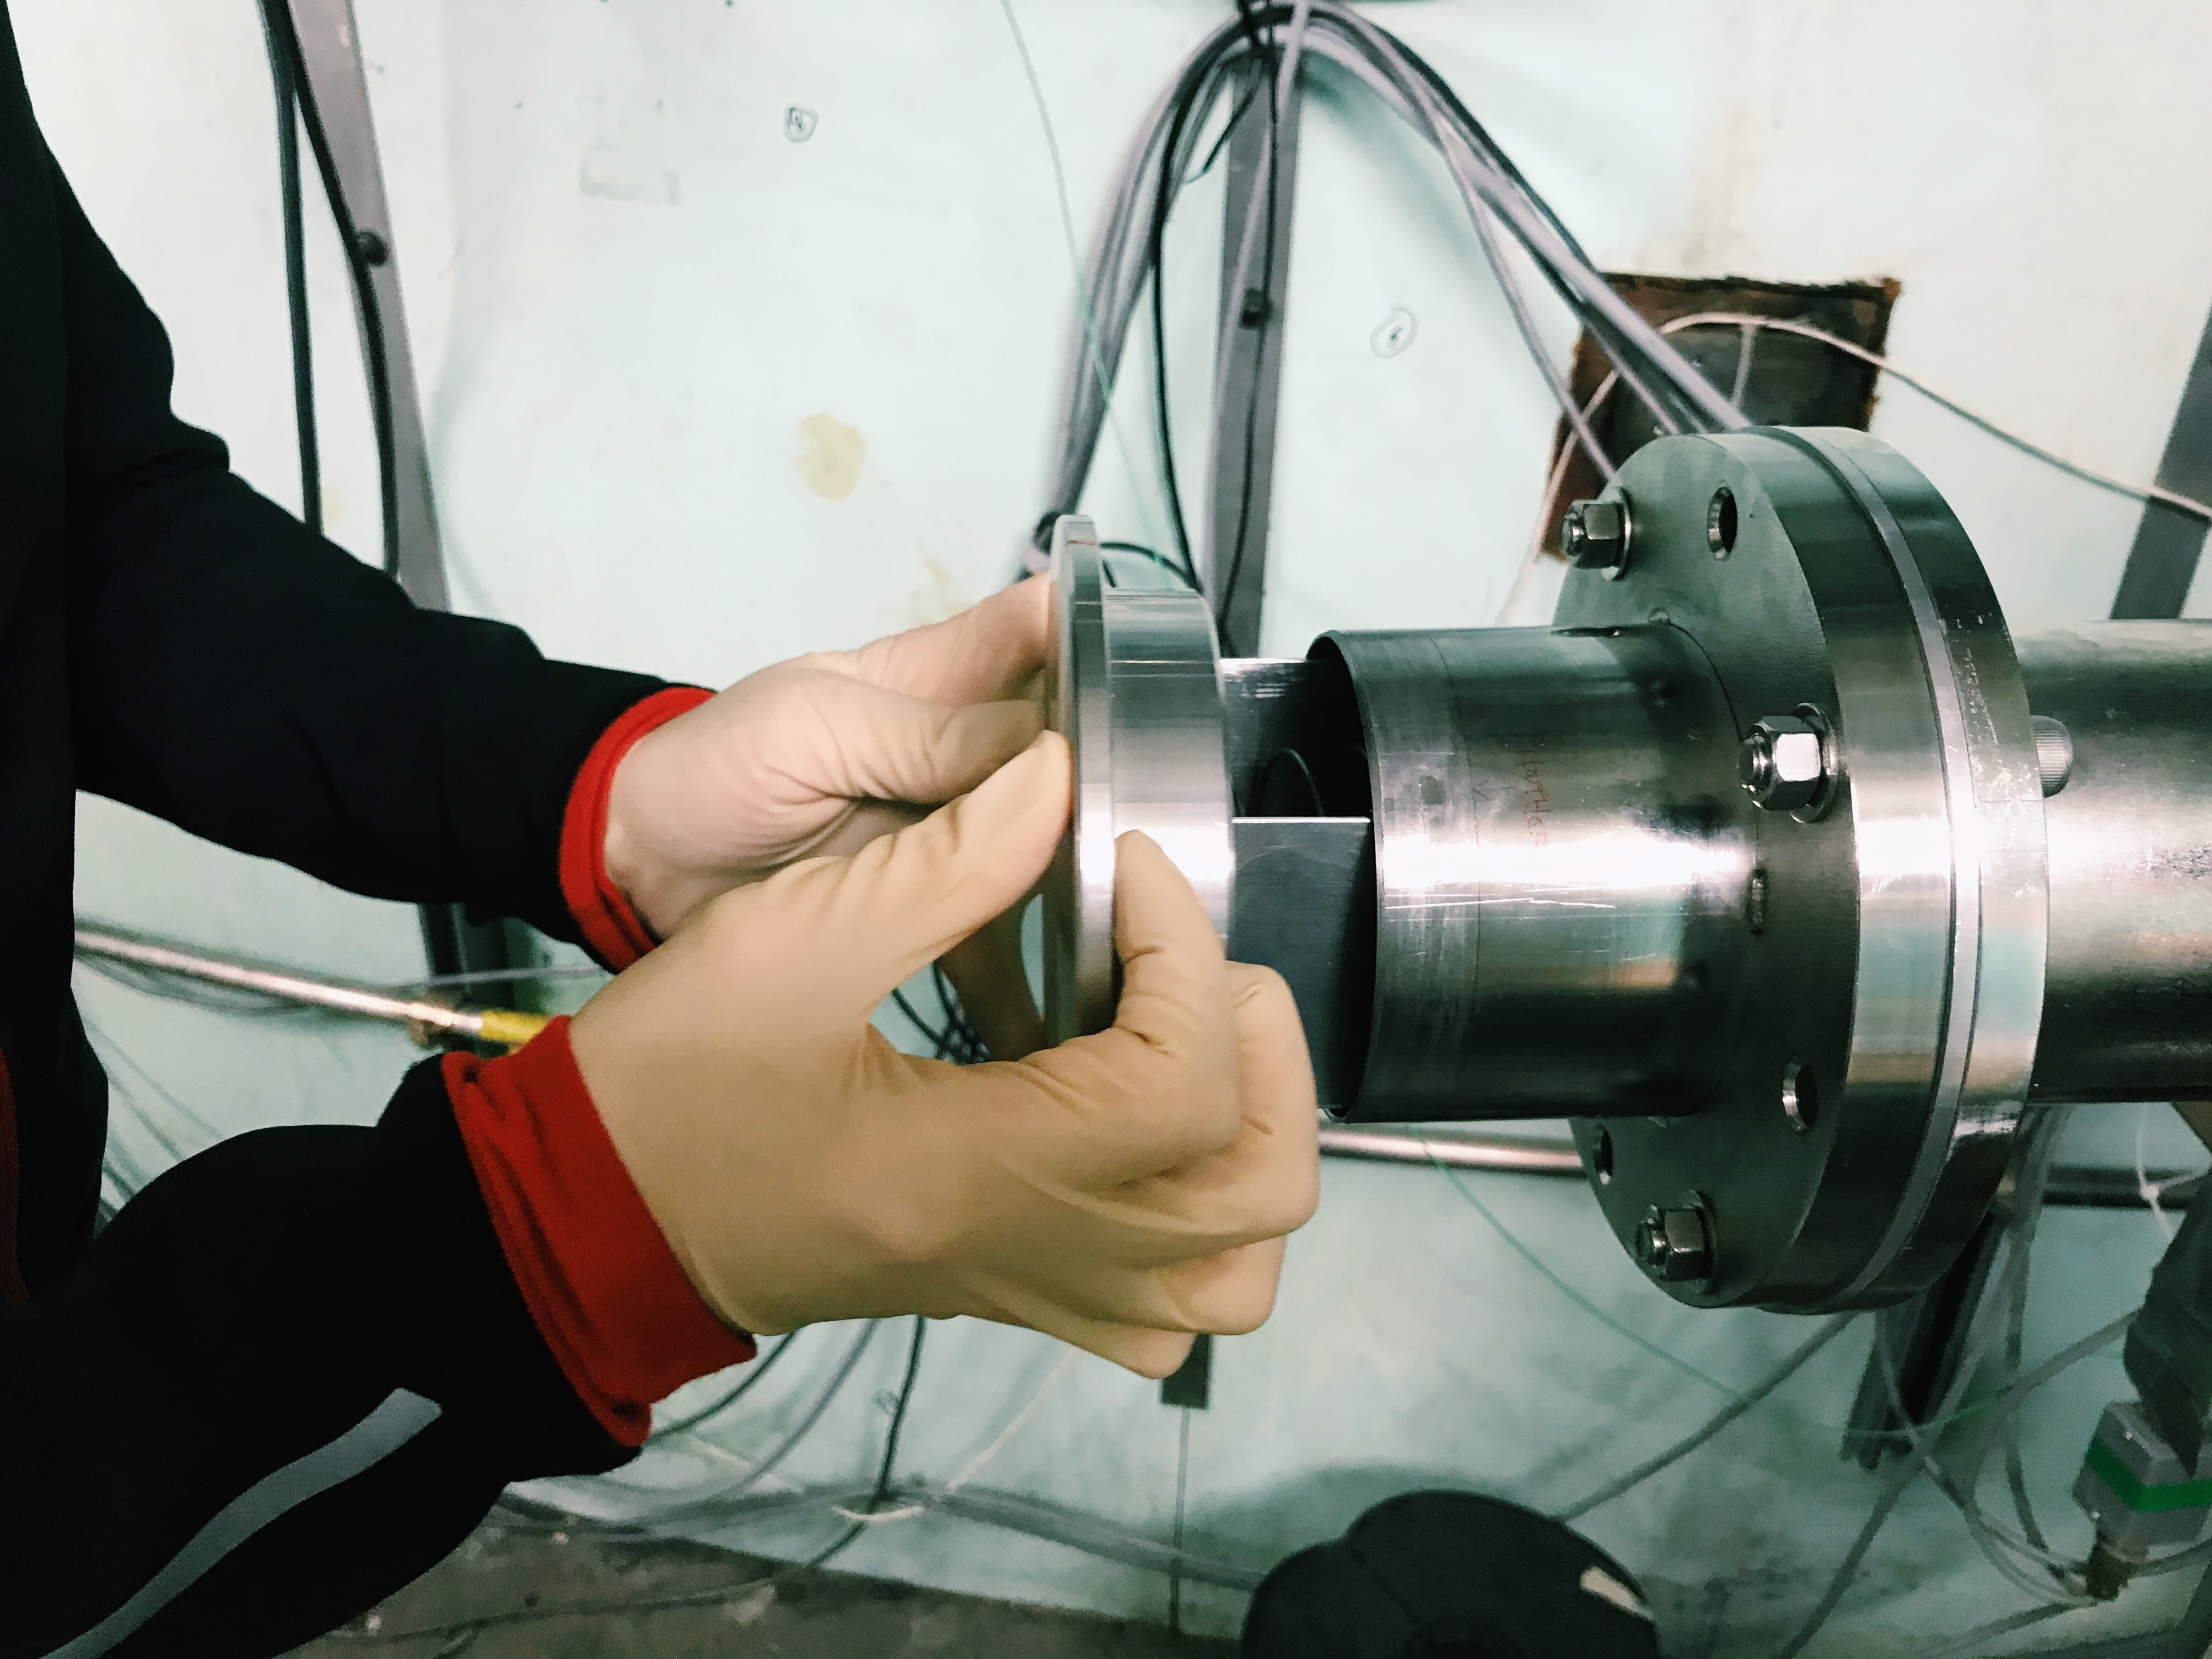
\includegraphics[width=\textwidth]{tube.JPG}
        \caption{Beam tube}
        \label{fig:tube}
    \end{subfigure}
    ~ %add desired spacing between images, e. g. ~, \quad, \qquad, \hfill etc. 
    %(or a blank line to force the subfigure onto a new line)
    \caption{The figure shows the finished stacked target, on how it was placed in the tube. }\label{fig:finished_stack}
\end{figure}
\noindent
The target was irradiated for exactly an hour, and the current read of the beam integrator evenly, so assure it increases constantly. Beam current from beam integrator was 128.5 nA. Full scale amperes was $2\cdot 10^{-7} $ A. Right after end of beam, the targets were sealed in small plastic bags to avoid contamination, and counted immediately. 

%Setup (cyclotron, caves, bending magnets, faraday cup, beam integrator, vacuum)

\subsection{Beam profile}
The stainless steel in the front and back of the target stack was attached to a gafchromic film after irradiation, and we were able to measure the actual beamprofile throgh the target stack. Due to scattering, the beam profile tends to broaden through the stack. However, the beam was stopped in the stack, hence the profile that was measured is not valid for the spread in the stack. \textcolor{red}{Image-J\footnote{https://imagej.nih.gov/ij/download.html} is an imaging process program that allowed us to measure the beam spot, finding the relative intensity of the beam spot on the gafchromic films. Radius of the activity from stainless on gafchromic film is used in program Image-J. The intesity profile is Gaussian, and the beamprofile had a full width half maximum of ...., and in the back was .... }. By measuring the beam profile, we were able to build confidence in the size of the beam spot. The stainless steel \textcolor{red}{(which consist of )} has fast decay time. It emits beta particles. Since beta particles do not emit straight, thus the actual beam spot is slightly smaller.   

\subsubsection{Counting on detectors}
Since counts are based upon Poisson statistics, \textcolor{red}{check notes!!!}, the more counts each peak has, the better statistics. Right after end of beam all the foils were counted for a short period of time to assure to measure the short-lived activities. Since the decay-rate for these nuclei are high, the statistics were ok. The longer after end of beam, the longer counts to assure good statistics for the longer-lived products. The foils were counted for a period of 4 weeks after end of beam. Backgrond spectra were taken for each detector as well. This was especially important for detectors 1-6 which were located in cave 4C, where background was present. 


\chapter{Analysis}

\subsection{Theory on radioactivity and production}

\subsection{Statistics}

\subsection{Efficiency curves}

\section{Gamma-ray spectroscopy}

FitzPeakz was used to find peaks in each spectra. From each spectrum, FitzPeakz provided a report file with the detector the correct detector calibration, datetime, livetime. For each peak, a peak energy, centre channel, full width half maximum of the peak, significanse, goodness of fit, peak area, uncertainty in peak area, gammas per second, and uncertainty in gammas per second, and an backgrond estimation was provided. The most important parameters were the energy and peak area ($N_C$), along with uncertainty in peak area. Gammas per second (also called count rate) was used get an indication of the rate of gammas, which in cases where backgrond was a question, a comparison along with background spectra could determine whether we needed to do a background subtraction.  \\

\noindent 
A program ran through all report files for each target, and gave a list of energies within a tolerance. If the energies were \textcolor{red}{within a tolerance of 0.5 keV??}, then energies were averaged.  On The Lund/LBNL Nuclear Data Search \footnote{http://nucleardata.nuclear.lu.se/toi/}, energies could be searched for within a tolerance for mass numbers ranging from the lowest stable isotope of the target - approximately 12 (which was calculated via the Q-value for possible reactions with 33 MeV deuterions) and up to two mass numbers (1 deuterions with one proton and one neutron) from the highest stable isotope. Each of the energies were tested and most assigned to a nucleus. 

\subsection{Background subtraction}

\noindent 
In a few number of cases, background subtraction was necessary, due to the presence of some nuclei in the background. \textcolor{red}{This was especially necessary for some isotopes of Cobalt, which are high in production for both nickel and iron. Other background??}. The general rule of thumb was only to use background subtraction when all gamma lines for the nucleus was also present in the background with a count rate of the same order. If it was only a shared gamma line, we would try to avoid using it at all. \\

\noindent 
The calculation was done the following way: 
Countrate is defined as the number of counts divided by the livetime of the spectrum, in units counts/second. 
$$C=\frac{N_C}{\Delta t_\text{live}}$$
The number of observed counts is the sum of the true gammas and the background. 
\begin{equation}
    C_\text{observed}=C_\text{true} + C_\text{background}
\end{equation}

\begin{equation}
    C_\text{observed} = \Big(\frac{N_\text{true}}{\Delta t_\text{live}} \Big)_\text{current spectrum} + \underbrace{\Big( \frac{N_\text{background}}{\Delta t_\text{live}} \Big)}_\text{=constant} _\text{background spectrum}
\end{equation}


From above we have that 
\begin{equation}
    N_\text{observed}=C_\text{observed}\Delta t_\text{live} = \Delta t_\text{live}(C_\text{true}+C_\text{background})
\end{equation}
\begin{equation}
    C_\text{true} = C_\text{observed}-C_\text{background}
\end{equation}

Finally, the true number of counts is

\begin{equation}
    N_\text{true}=N_\text{obs}- (\Delta t_\text{live} C_\text{background})
\end{equation}


\subsection{Cross section}
\begin{equation} \label{eq:CS_ch3}
    \sigma(\langle E \rangle) = \frac{A_0}{N_T \Phi (1-e^{-\lambda \Delta t_\text{irr}})}
\end{equation}


\subsection{Activities}
The following section is based on Krane chapter 6\footnote{https://faculty.kfupm.edu.sa/phys/aanaqvi/Krane-Ch-6.pdf}: \\

\noindent 
The activity of a radioactive nucleus is equal to the radioactive decay rate 

\begin{equation}
    A = \frac{dN}{dt} = -\lambda N
\end{equation}
\noindent where N is the number of nuclei, t is the time and $\lambda$ is the decay constant. If we assume a target of a stable nucleus, which is exposed to a particle beam which induces various nuclear reactions, the constant rate of production of a specific reaction is dependent on the number of target nuclei, the current of flux of the particle beam and the reaction cross section 
\begin{equation} \label{eq:prod_rate}
    R = N_T \Phi \sigma
\end{equation}
\noindent 
where R is the production rate, $N_T$ is the number of target nuclei, $\Phi$ is the beam current or flux, and $\sigma$ is reaction cross section. In the assumption of the production rate being a constant value, the number transformed target nuclei is small in comparison to the total number during the irradiation time. The number of produced nuclei from a specific reaction is thus 

\begin{equation}
    dN = Rdt -\lambda N dt
\end{equation}

\noindent which has the solution 

\begin{equation}
    N(t) = \frac{R}{\lambda} (1-e^{-\lambda t})
\end{equation}

\noindent The total activity produced is thus 
\begin{equation}
    A(t) = R(1-e^{-\lambda t})
\end{equation}

\noindent When a target is irradiated, the activity of the product nucleus will increase until \textit{secular equilibrium} is achieved, which is when the product rate and decay rate are constant. Hence it is not necessary to irradiate a target for more than 2-3 half lives. \\ 

\noindent It is common that a radioactive nucleus decay into another radioactive nucleus. Hence the daughter activity will increase due to feeding from the parent. For multiple decay, \textit{Bateman equation} is used describing the activity in nucleus n of the decay chain \textcolor{blue}{(Voyles2018)}.

\begin{equation} \label{eq:Bateman}
    A_n(t) = \lambda_n \sum_{i=1}^{n} \Big[ \Big(N_{i,0} \prod_{j=i}^{n-1}\lambda_j\Big) \cdot \Big( \sum_{j=i}^{n}\frac{e^{-\lambda_j t}}{\prod_{i\neq j}^{n}(\lambda_i - \lambda_j) }\Big) \Big]
\end{equation}

\noindent 
where $A_n$ is the activity of nuclei n in the decay chain, with the corresponding decay constant $\lambda_n$. The equation sums over all nuclei in the decay chain. $N_{i,0}$ is the initial number of nucleus i, and j is the nucleus which is feeding into nucleus i.




\subsubsection{End of beam activities}
From equation \ref{eq:CS_ch3}, we need to estimate the end of beam activity for each nuclei. The end of beam activities were estimated using curvefit of multiple gamma-rays measured at different time points after end of beam. The activity measured a time t is calculated using one gamma-ray
\begin{equation} \label{eq:activity_spectra}
    A(t)=\frac{N_C \lambda}{\epsilon I_\gamma (1-e^{-\lambda \Delta t_\text{live}})e^{-\mu\rho\Delta r/2}}
\end{equation}
\noindent
where $N_C$ is the number of counts observed in the peak, $\epsilon$ is the detector efficiency, $I_\gamma$ is the intensity of the gamma-line, $\lambda$ is the decay constant of the nucleus, $\Delta t_\text{live}$ is the livetime of the spectrum. \textcolor{red}{The term $e^{-\mu \rho \Delta r/2}$ is the attenuation of the foil which is taken from \textcolor{red}{XCOM}, and $\rho\Delta r$ is a correction term due to thin foils which are not point sources, where we assume that only half of the mass density is detected since there is some attenuation in the foil as well.?????}.\\

\noindent 

\begin{enumerate}
    \item Activity 
    \item Uncertainty 
    \item Cumulative vs independent 
    \item False peaks
    \item Shared peaks and feeding. 
\end{enumerate}

\noindent
The scipy-curvefit method takes in all activities and uncertainties and minimizes the $\chi^2$ per degree of freedom, with an uncertainty weighting favouring the lowest uncertainties. \\

%\noindent 
%A decay chain is a decay where a parent product decays into a chain of daughter products, via $\alpha$ or $\beta$-decay. In the cases here, it is $\beta$-feeding. This means that the abundance of a particular isotope with feeding increases after the end of beam. 

\noindent 
If the first nucleus we observe in a decay chain has a parent that was produced but has too short half life to be observed, the first nucleus is reported as cumulative cross section. If there are independent observations in the next levels of the decay chain, they will be reported as independent and along with cumulative values.  

\noindent 
In the cases of this experiment, there was one step and two step decay that was calculated. With no feeding the simplest form of radioactive decay is sufficient

\begin{equation} \label{eq:radioactive_decaylaw}
    A(t)=\frac{dN}{dt}= \lambda N
\end{equation}

\noindent which simplies to when solving the differential equations

\begin{equation} \label{eq:onestep_activity}
    A(t) = A_0 e^{-\lambda t}
\end{equation}
\noindent 
In the cases of two step decay (n=2), the activity of the daughter is calculated from equation \ref{eq:Bateman}

\begin{equation} \label{eq:twostep_activity}
    A_2(t)= \lambda_ 2 \Big[ N_{1,0}\lambda_1 \frac{(e^{-\lambda_1} + e^{-\lambda_2})}{\lambda_1 - \lambda_2} + N_{2,0}e^{-\lambda_2 t}  \Big]
\end{equation}

\noindent from equation \ref{eq:radioactive_decaylaw}, the activity $A=\lambda N$, and two step decay is written as 

\begin{equation}
    A_2(t) = \frac{A_{1,0}\lambda_2}{\lambda_1-\lambda_2 } (e^{-\lambda_1 t} + e^{-\lambda_2 t }) + A_{2,0}e^{-\lambda_2 t}
\end{equation}

\noindent 
If the parent activity is known, the activity and cross section will be reported as independent and cumulative. If the parent activity is not known (due to lack of gamma lines for instance), the daughter activity and parent activity will be reported as cumulative. Figure \ref{fig:193mPt_activitycurve} shows an activity curve using single decay, for $^{193m}$Pt in foil 6. 

\begin{figure}
    \centering
    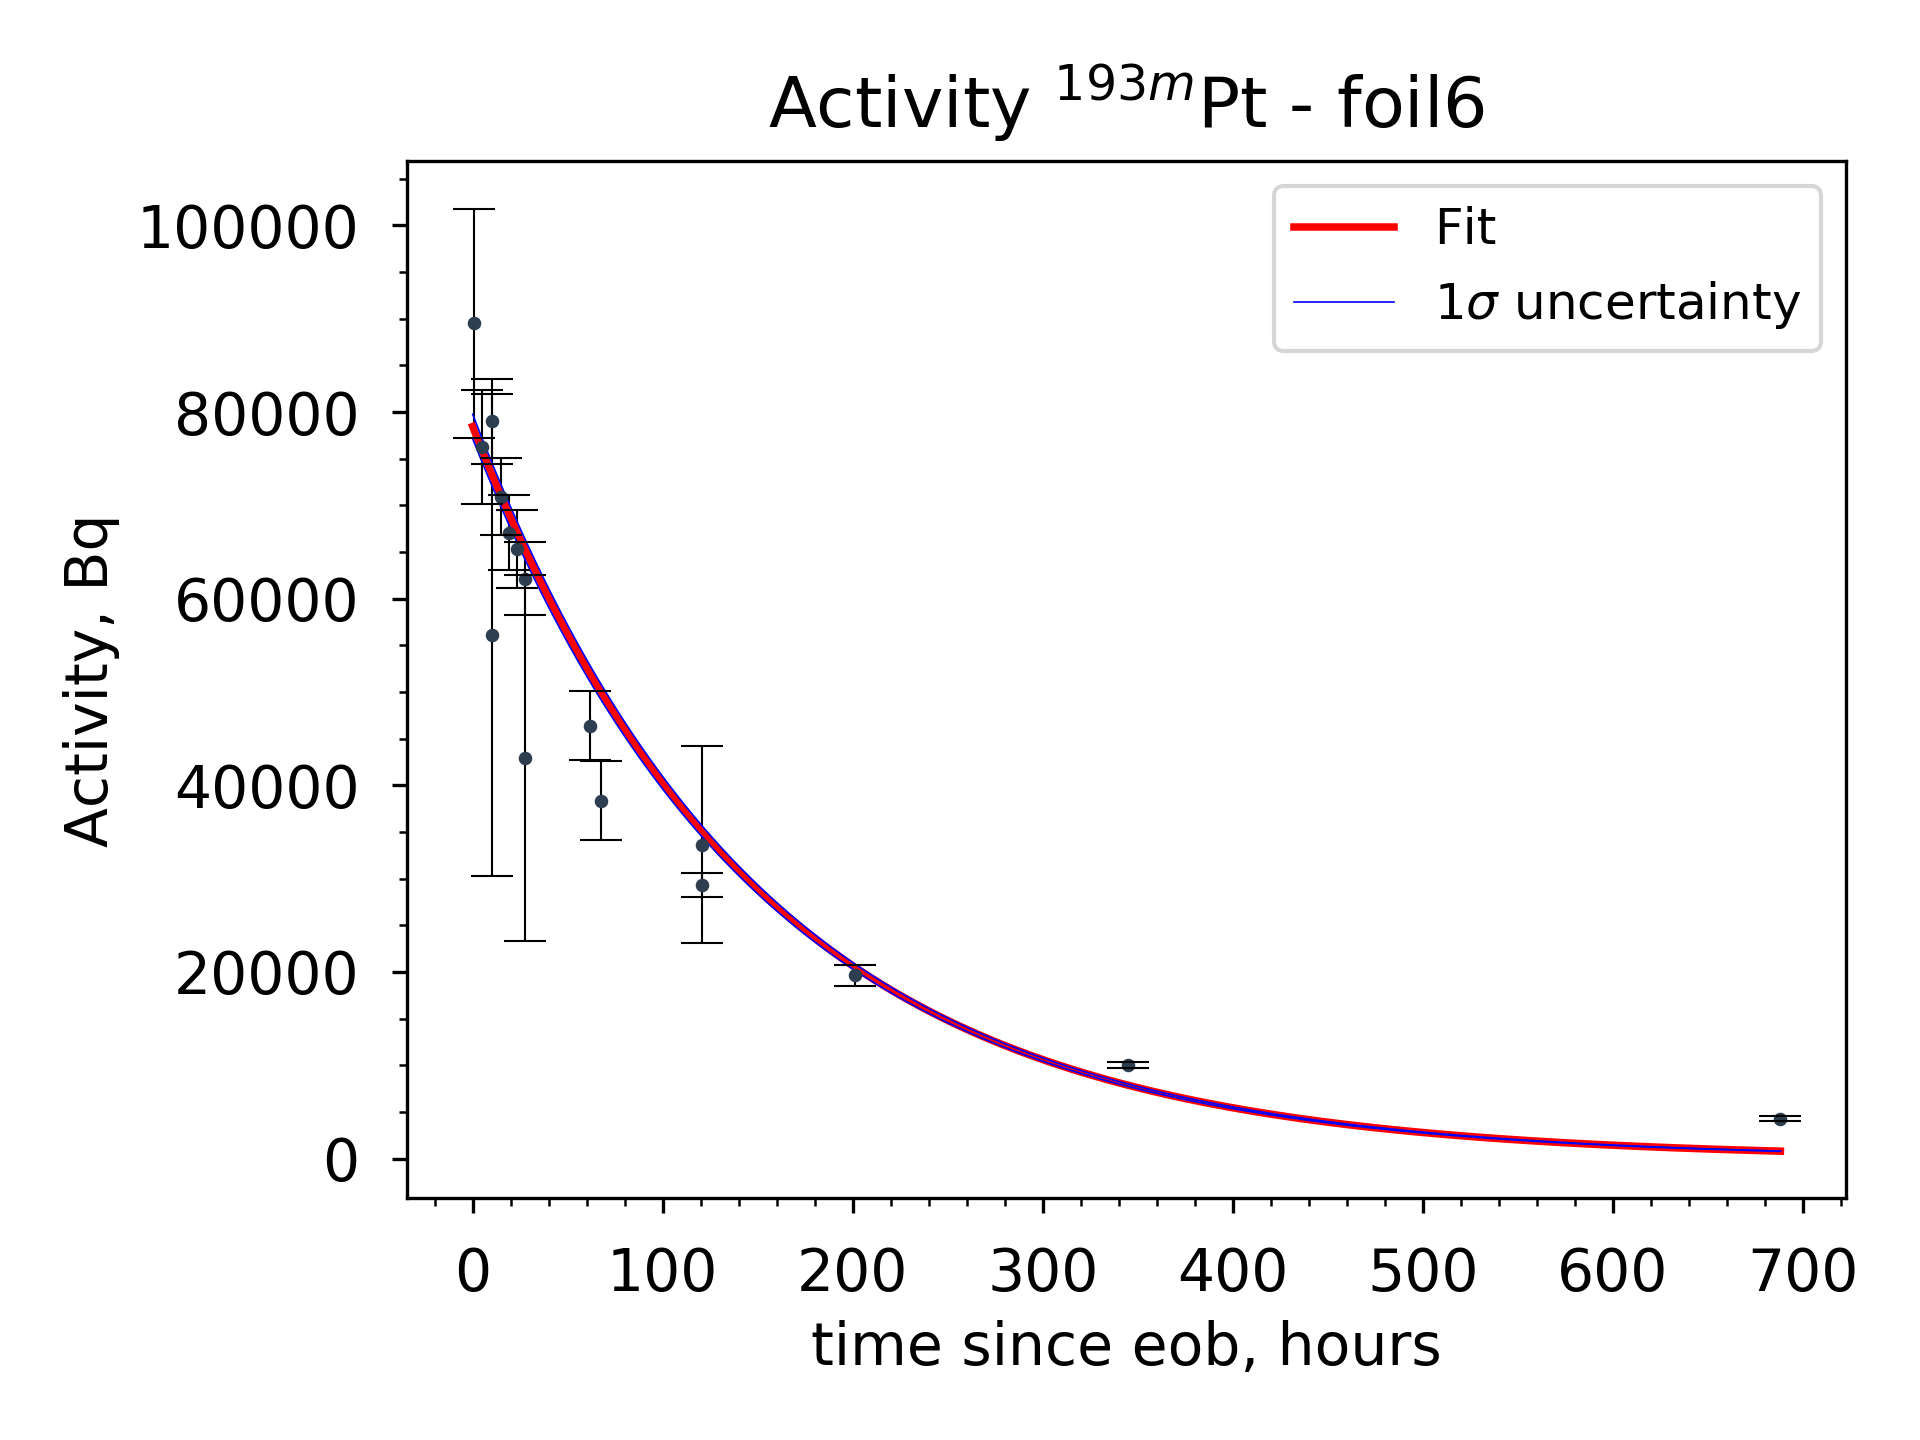
\includegraphics{_activity_193mPt_677.png}
    \caption{An example of an activity curve using foil number 6 of $^{193m}$Pt with activities measured from the gamma ray spectroscopy using equation \ref{eq:activity_spectra}. The fitted curve is the single decay \textcolor{red}{Include two step decay also to give an example. } }  
    \label{fig:193mPt_activitycurve}
\end{figure}


\subsection{Beam Current}

The beam integrator gave a current of tube hitting the stack with 128.5 nA. However, due to the large energy degradation in the energy stack, there will be a certain spread in the beam, following scattering. This is also the first experiment which have used deuterium on a stack of targets, so beforehand, we did not know how much deuteron break-up would affect the current throughout the stack. Reactions from the copper, nickel and iron foils were used as monitor reactions to estimate the weighted average beam current which was used in the cross section calculation in equation \ref{eq:CS_ch3}. Well-known cross sections from IAEA were used\footnote{https://www-nds.iaea.org/medical/monitor_reactions.html. Need to add citation for each datapoint used.}; $^{\text{nat}}$Fe(d,x)$^{56}$Co, $^{\text{nat}}$Ni(d,x)$^{56,58}$Co and $^{\text{nat}}$Cu(d,x)$^{62,63,64}$Zn. \textcolor{red}{This method provides a more sensitive beam current calculation}. \\ 

\noindent 
In order to calculate the cross sections, we need an accurate measure of the beam current. Thus, with well-known cross sections from the monitor reactions, we can estimate the beam current: 

\begin{equation} \label{eq:BC_nodiff}
    \Phi = \frac{A_0}{N_T (1-e^{-\lambda \Delta t_\text{irr}})\sigma(\langle E\rangle)}
\end{equation}

\noindent 
In cross section experiments\footnote{based on special curriculum, p. 14}, the suggested value is a \textit{flux average cross section}, which implies that the cross section is dependent on the flux-weighted average beam energy. One single foil thus provides one cross section measurement, with the energy uncertainty only being dependent on the energy distribution in each foil. For thin targets, we assume a stopping power $dE/dx=0$ (a good approximation for targets which are less than 50 mg/cm$^2$ \textcolor{red}{citation?}), hence we can replace the cross section in equation \ref{eq:BC_nodiff} with the normalized 

\begin{equation}
    \sigma(\langle E \rangle) = \frac{\int \sigma(\langle E \rangle) \frac{d\phi(\langle E \rangle)}{dE}dE}{\int \frac{d\phi(\langle E \rangle)}{dE}dE}
\end{equation}

\noindent where $\sigma(\langle E \rangle)$ is the well-known monitor cross section from IAEA, $\phi/dE$ is the differential deuterium fluence.  Using the above expression, beamcurrent can be written on the form 

\begin{equation}
    \Phi(\langle E \rangle) = \frac{A_0}{N_T (1-e^{-\lambda \Delta t_\text{irr}})\frac{\int \sigma(\langle E \rangle) \frac{d\phi(\langle E \rangle)}{dE}dE}{\int \frac{d\phi(\langle E \rangle)}{dE}dE}}
\end{equation}

\noindent 
The energy degradation was measured using NPAT's (nuclear physics analysis tool) Ziegler simulation. The code is based on Ziegler stoppingpower formalism and Monte Carlo simulations \textcolor{red}{Write more about npat, and what type of formalism its based on}. However, the large challenges to the simulation is to assign the correct energy bins. Especially, in energy ranges where the cross section is very sensitive to changes (changes rapidly as a function of energy). Figure \ref{fig:Ir_Flux_Distr} shows the energy distribution in the foils, where the flux is along the y-axis. The further back in the stack the harder it is to model, hence the full width half maximum increases

Thus, a need of variance minimization was necessary to assure that the correct energy bins was assigned to the stack. 

\begin{figure}
    \centering
    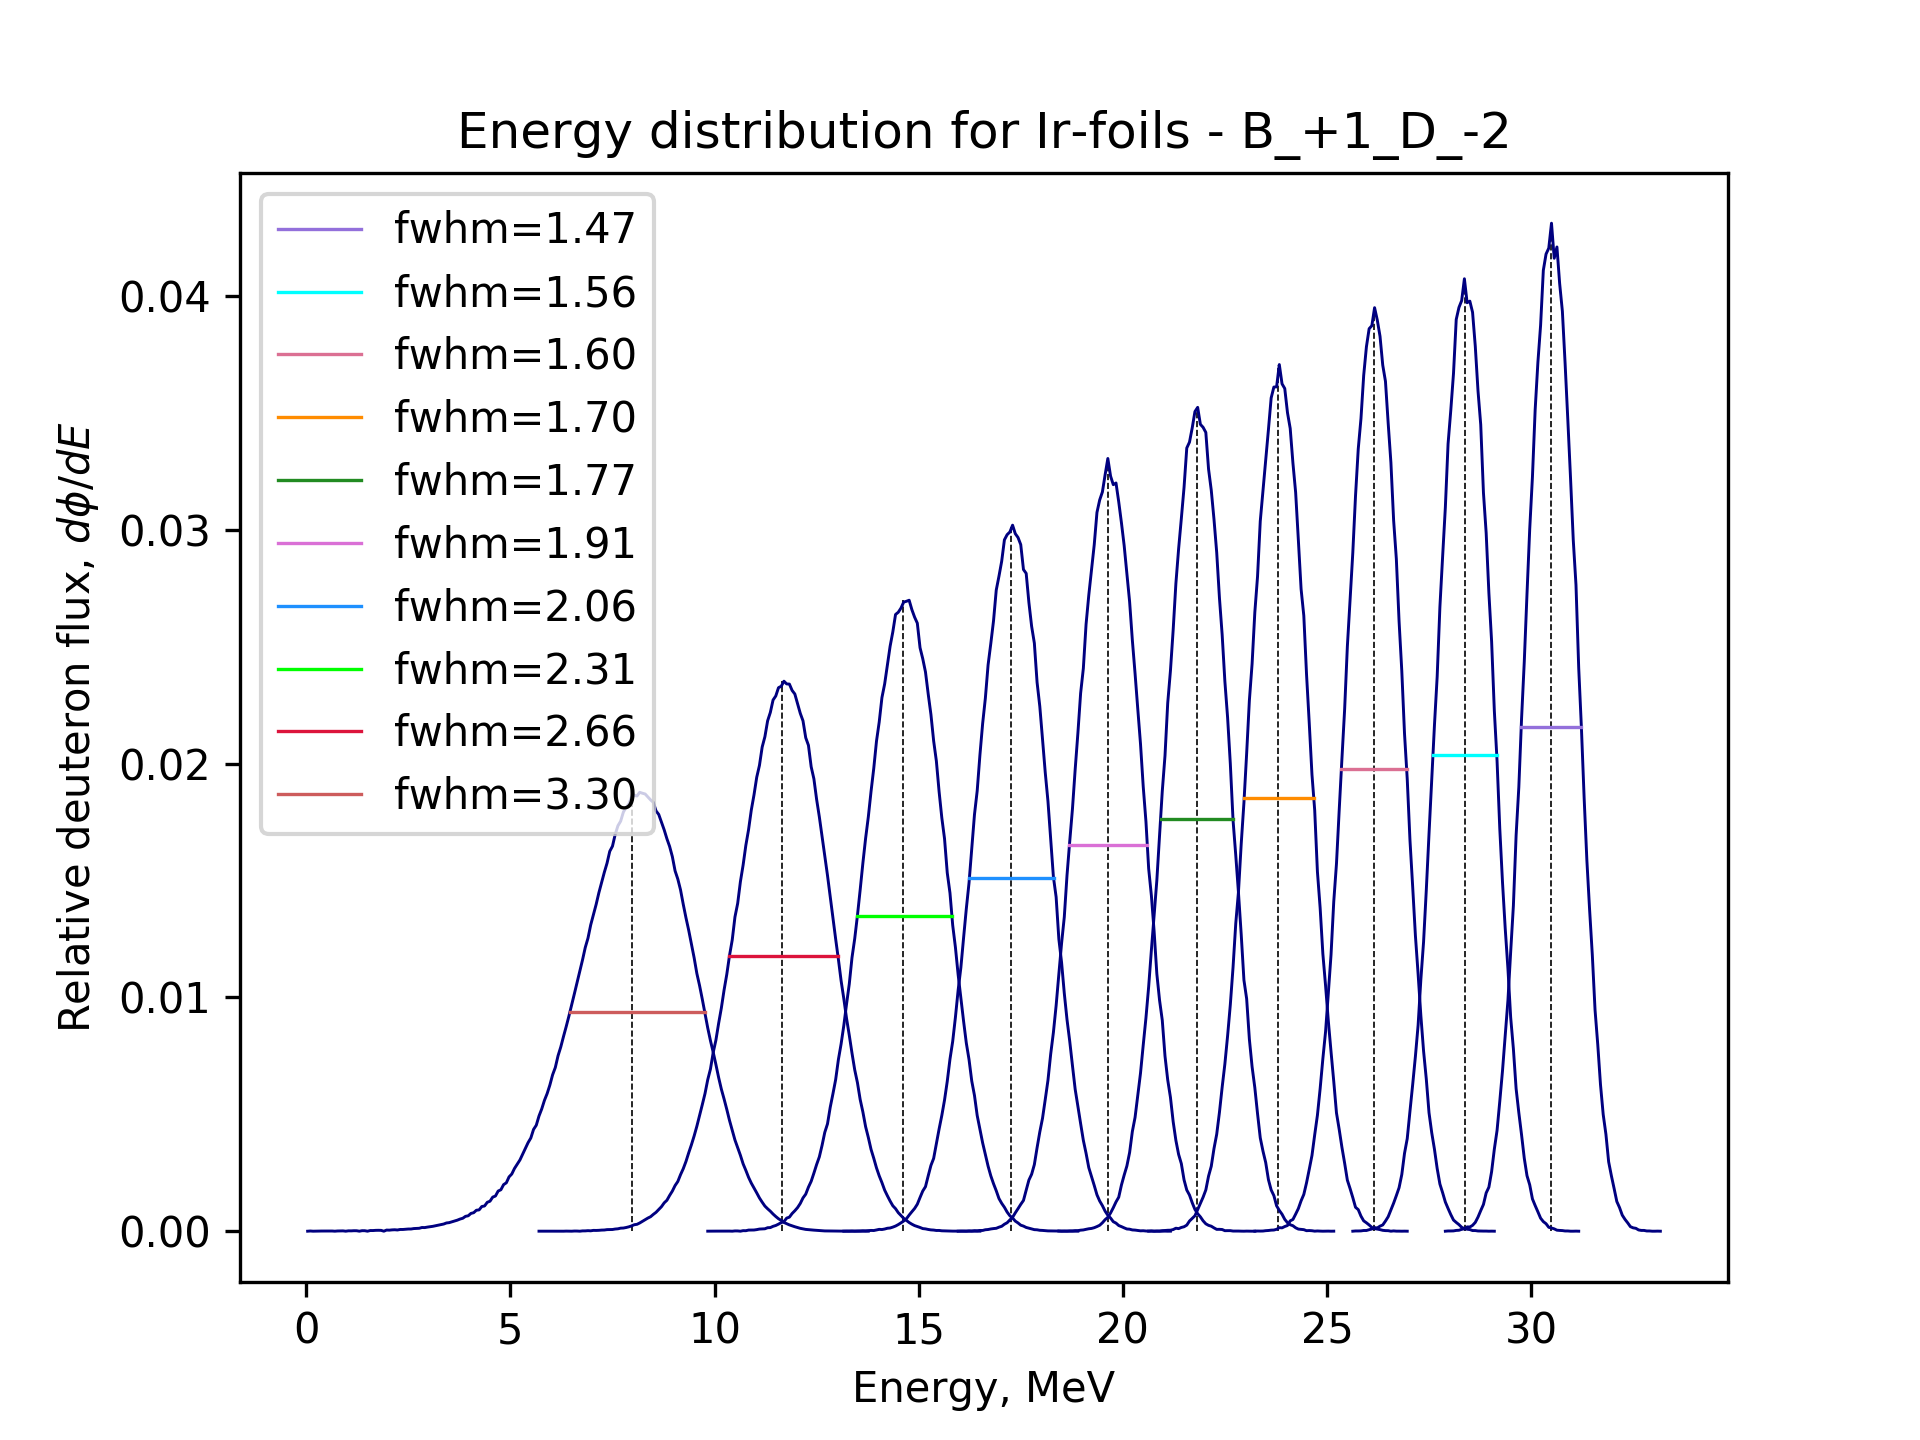
\includegraphics{Ir_flux_distribution_B_+1_D_-2.png}
    \caption{The energy distribution of the iridium foils throughout the stack. \textcolor{red}{Should be very sure that it the beamcurrent in the end. } }
    \label{fig:Ir_Flux_Distr}
\end{figure}


\subsection{Variance minimization}
Ziegler files provides a set of energy and fluxes through the different foils. 
Did a areal density and beam energy increase and dicrease to see how it affected the current. Gives an energy distribution. Show figures.  \\

$\chi^2$ is an estimation of the goodness of fit which weight includes weight of error. The value is divided on the number of degrees of freedom (essensially the number of parameters minus 1. \textcolor{red}{why?})
\begin{equation} \label{eq:chi_squared}
    \chi^2 = \sum_{i}^n \Big(\frac{ y_i - \overline{y}}{ \sigma_i} \Big)^2 
\end{equation}

\noindent 
The idea was to get an estimation of the values of $\chi^2$ over the different compartments (one compartment is one set of foils, for instance Ni01, Ir01, Fe01 and Cu01). Compartment 3, 6 and 9 was investigated to get an idea of the scaling parameter that gave lowest values. If we cared about the $\chi^2$ values at high energies (early in the stack), the currents tend to be bad in the back of the stack, due to scattering at compartment 3 being low. However, in compartment 3, we had 7 independent measurements of beam current which gave more data. In compartment 9, a lot of the currents were low due to most reactions being at the energy threshold. Hence compartment 6 was used, which had 5 measurements (61Cu, 56,58Co, 63,65Zn). 62Zn was below threshold, and iron did not have any foil in compartment 6. The compartment can be seen in figure \ref{fig:varmin_comp6}. 

\begin{figure}
    \centering
    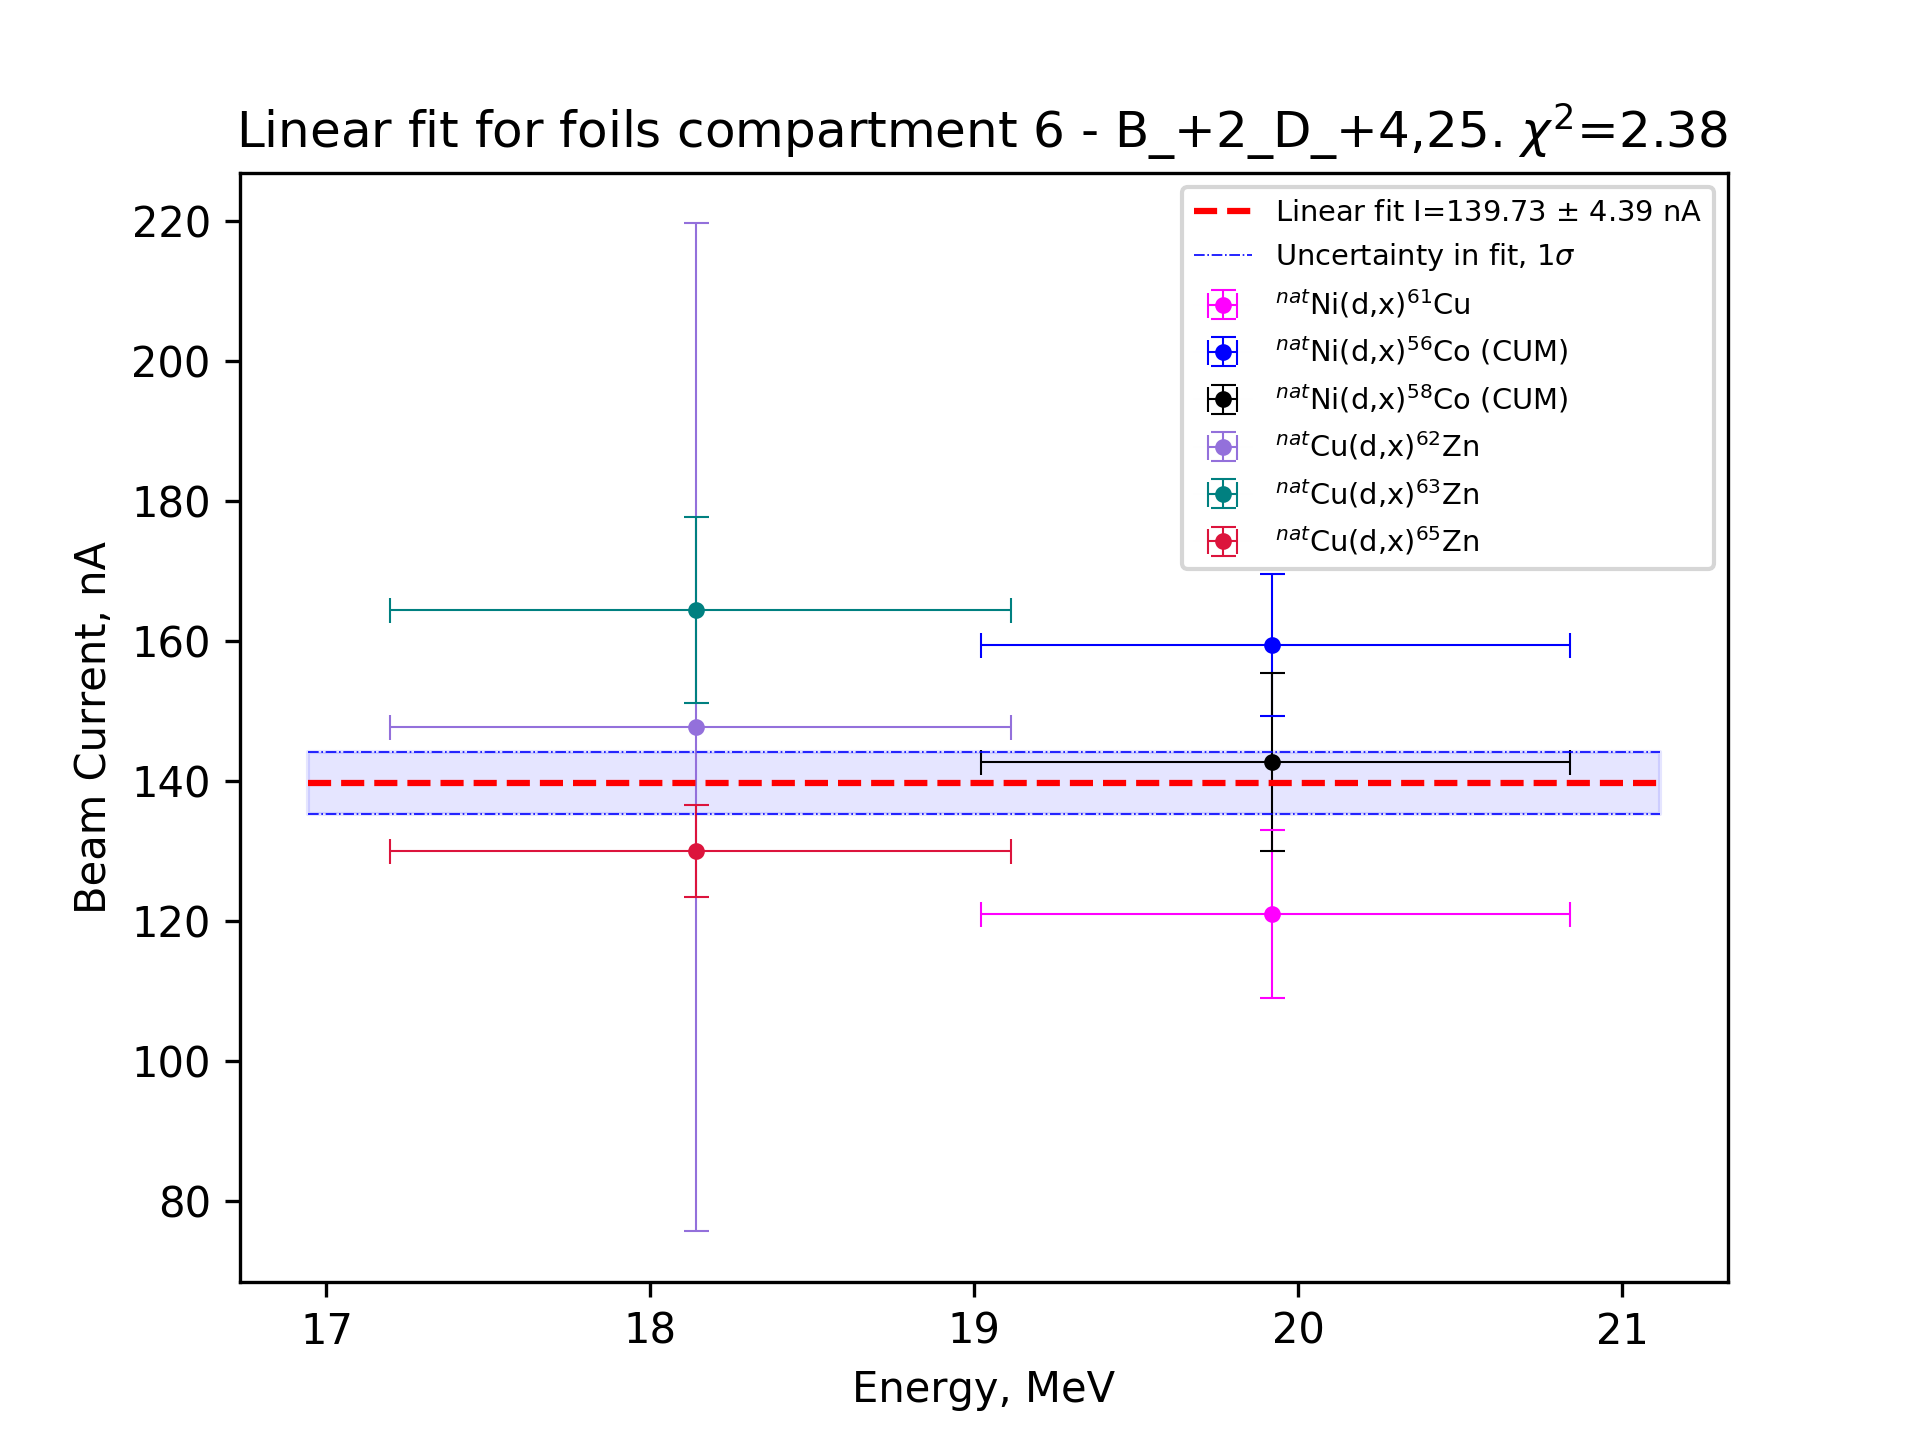
\includegraphics{minimization_6_B_+2_D_+4,25.png}
    \caption{Variance minimization in compartment 6.}
    \label{fig:varmin_comp6}
\end{figure}

Assuming constant beam current in one compartment. Hence we can have a linear fit between the beam current measurements. With no current degradation, $y=mx+b$, m=0, b is initial guess of 128.5 nA. 

\begin{figure}%
    \centering
    \subfloat[Before variance minimization]{{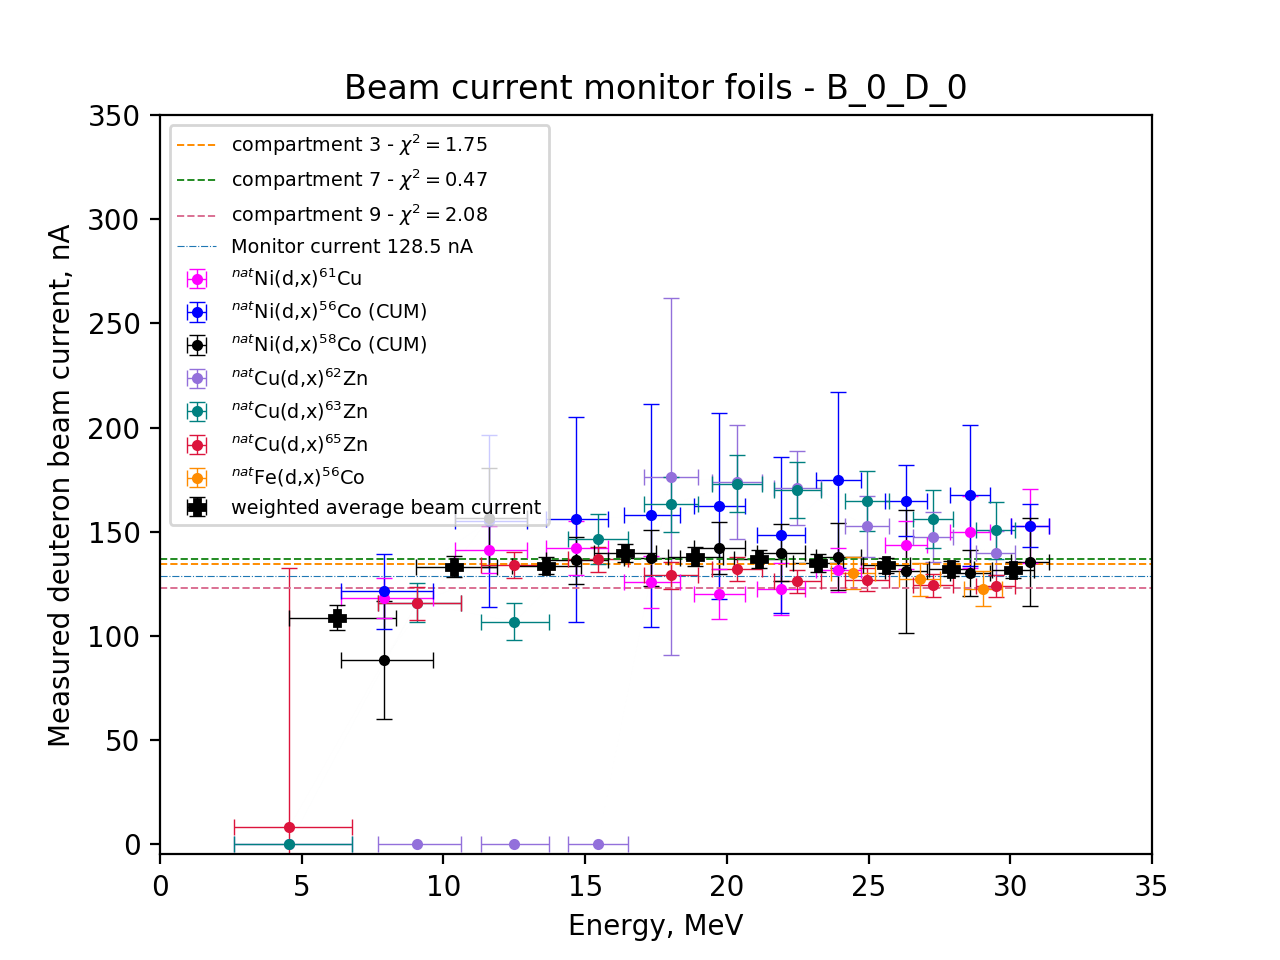
\includegraphics[width=8cm]{B_0_D_0.png} }}%
    \quad
    \subfloat[After variance minimization]{{\includegraphics[width=8cm]{B_+2,25_D_+5.png} }}%
    \caption{Before, the current in the back of the stack is tending to be lower. The $\chi^2$ in the different compartments also tend to be higher. After variance minimization, the values for $\chi^2$ are smaller and the estimated current in each compartment agrees more with each other. We do not expect much of current degradation.}%
    \label{fig:varmin_beamcurrent}%
\end{figure}


\subsubsection{The weighted averaged beam current, along with uncertainties}

Need to write statistical part first, about covariance matrix. 


Testing: the weighted average beam current for each target foil was used, to estimate the cross section. 

\begin{figure}%
    \centering
    \subfloat[]{{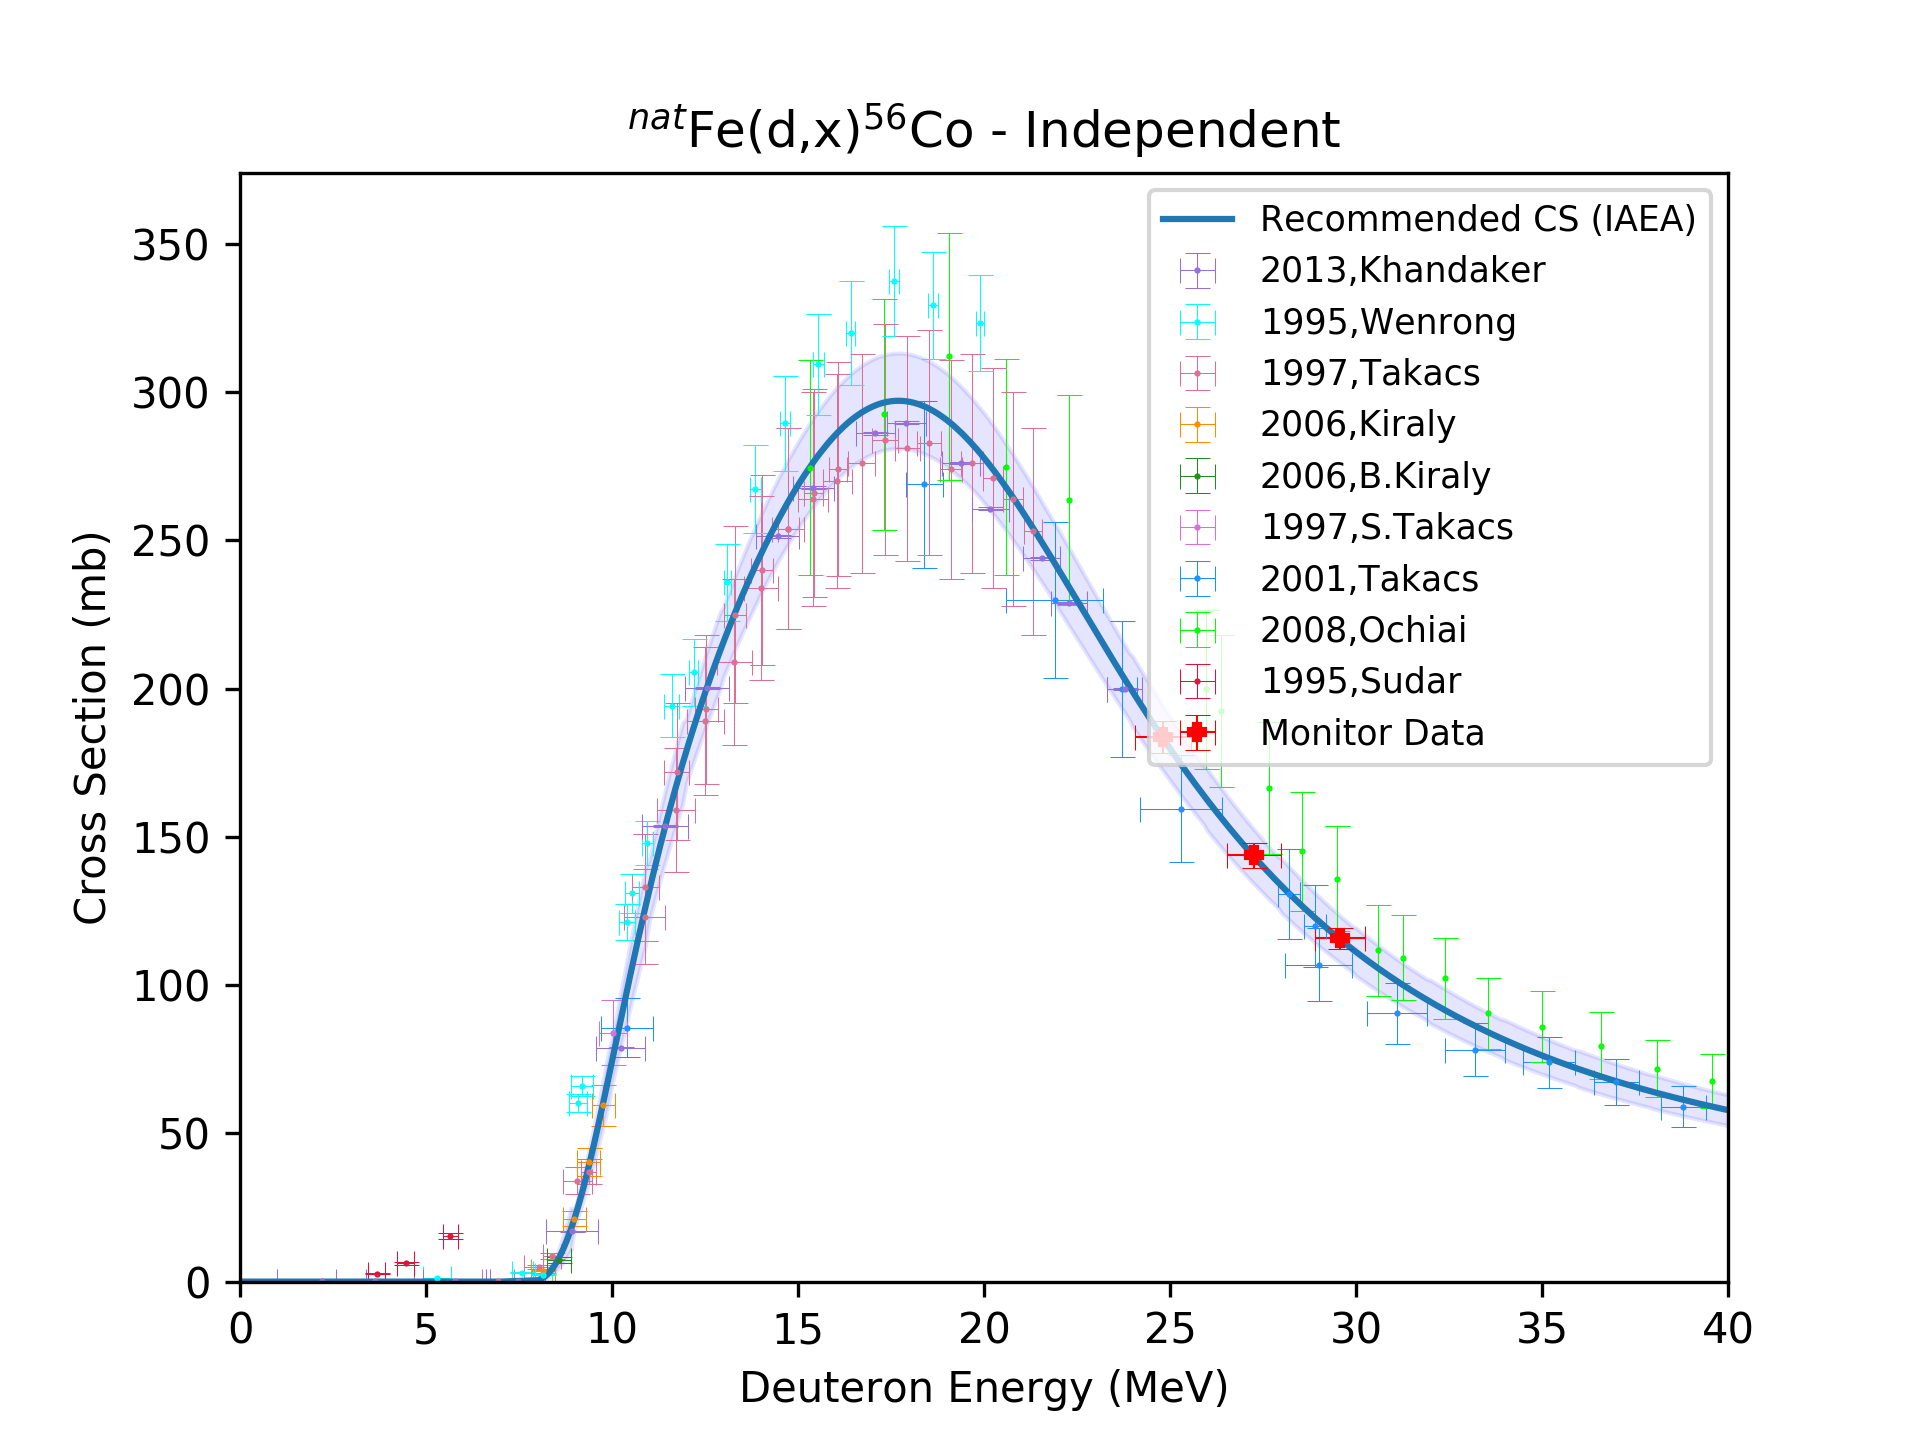
\includegraphics[width=5cm]{Fe_56Co.png} }}%
    \quad
    \subfloat[]{{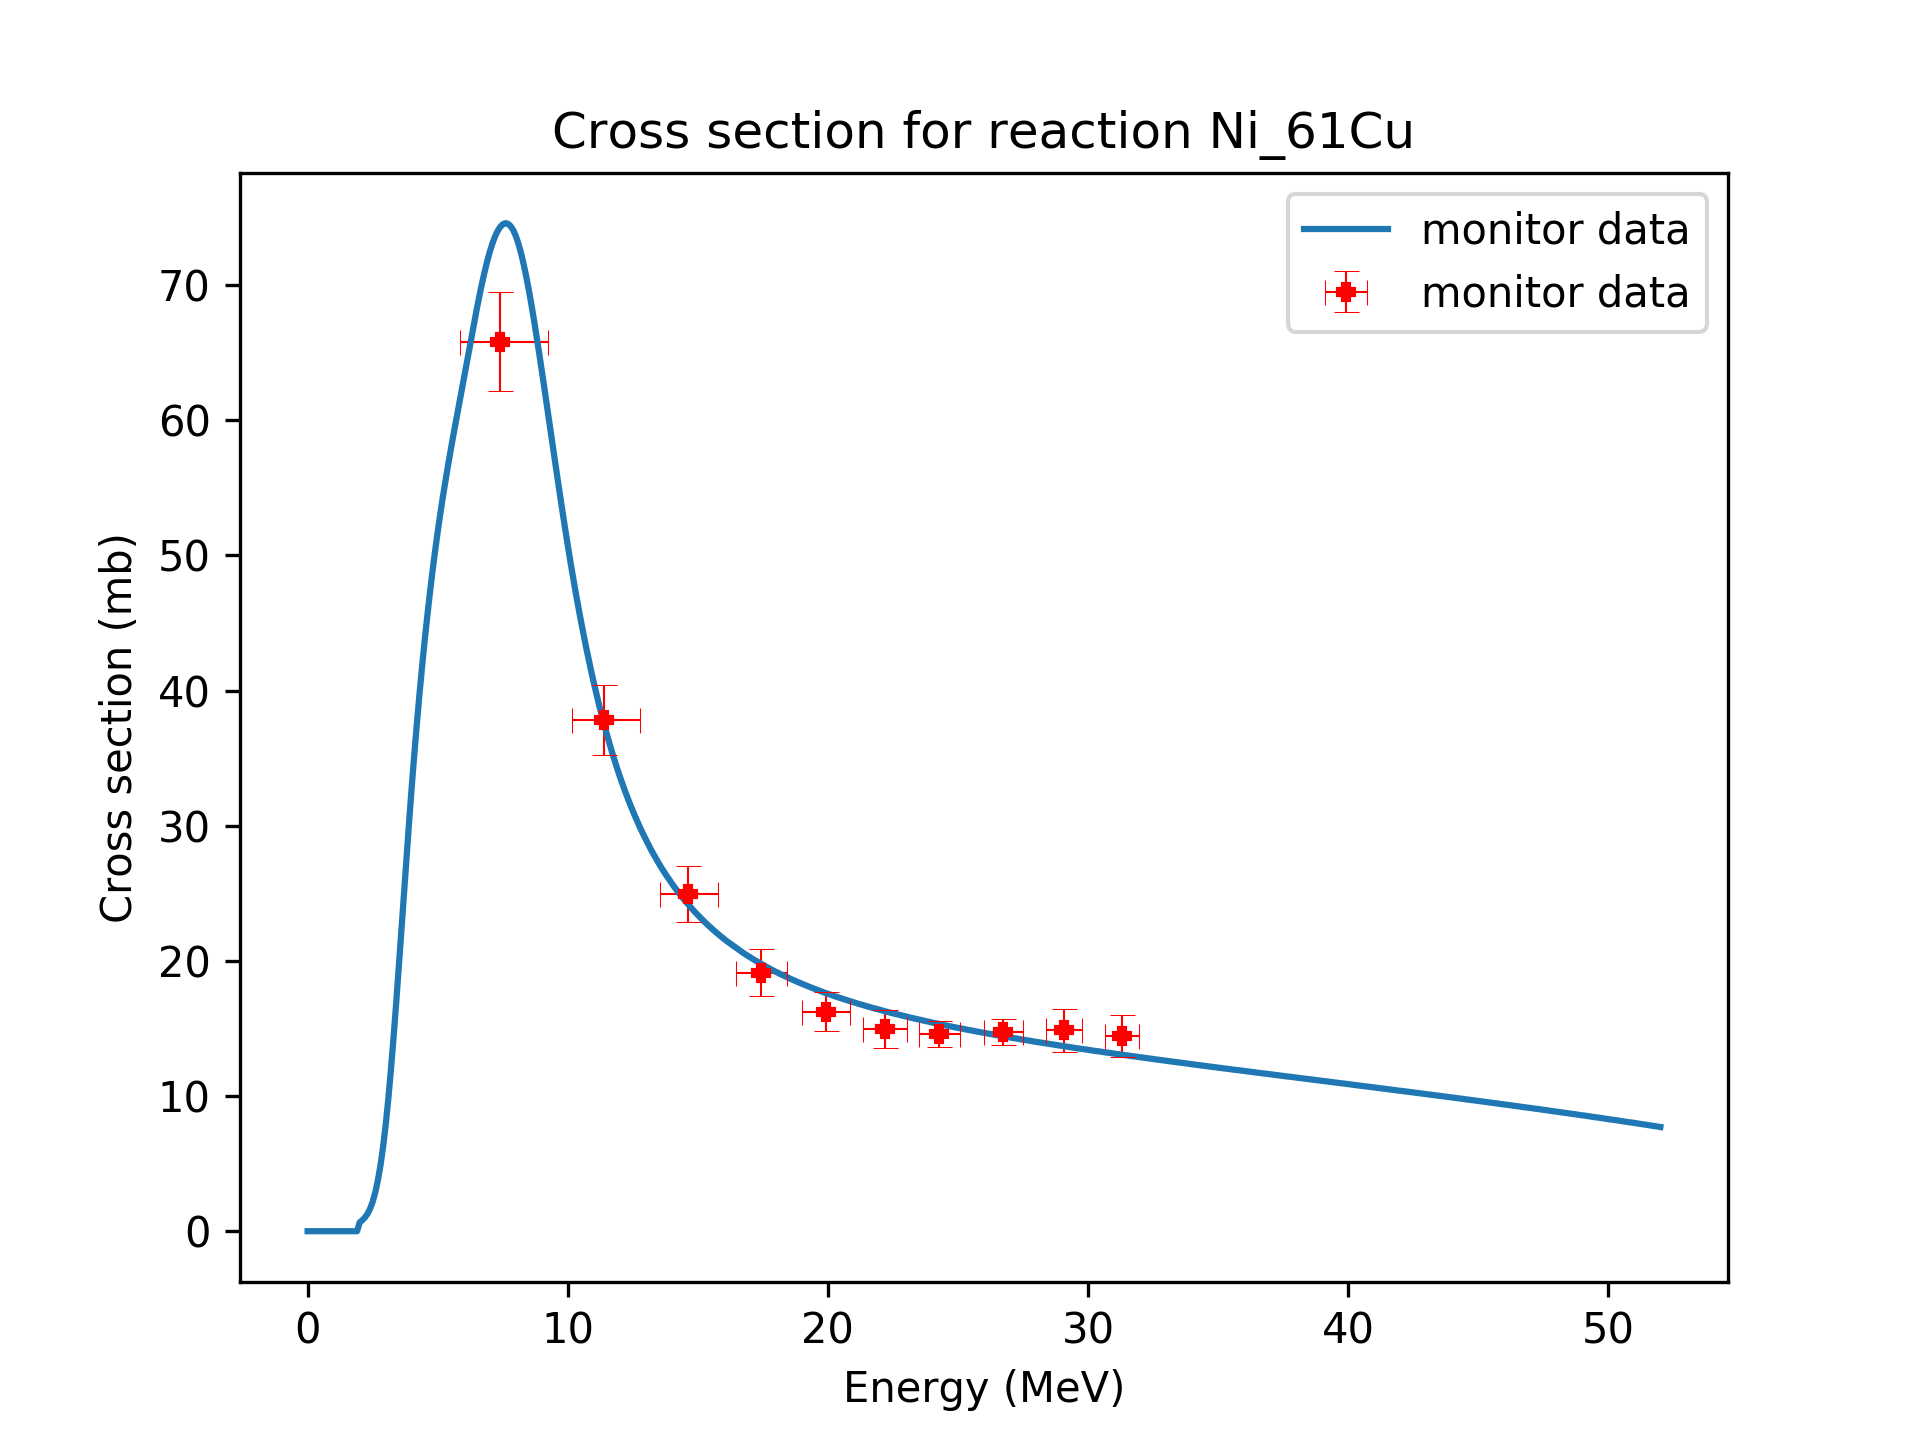
\includegraphics[width=5cm]{Ni_61Cu.png} }}%
    \subfloat[]{{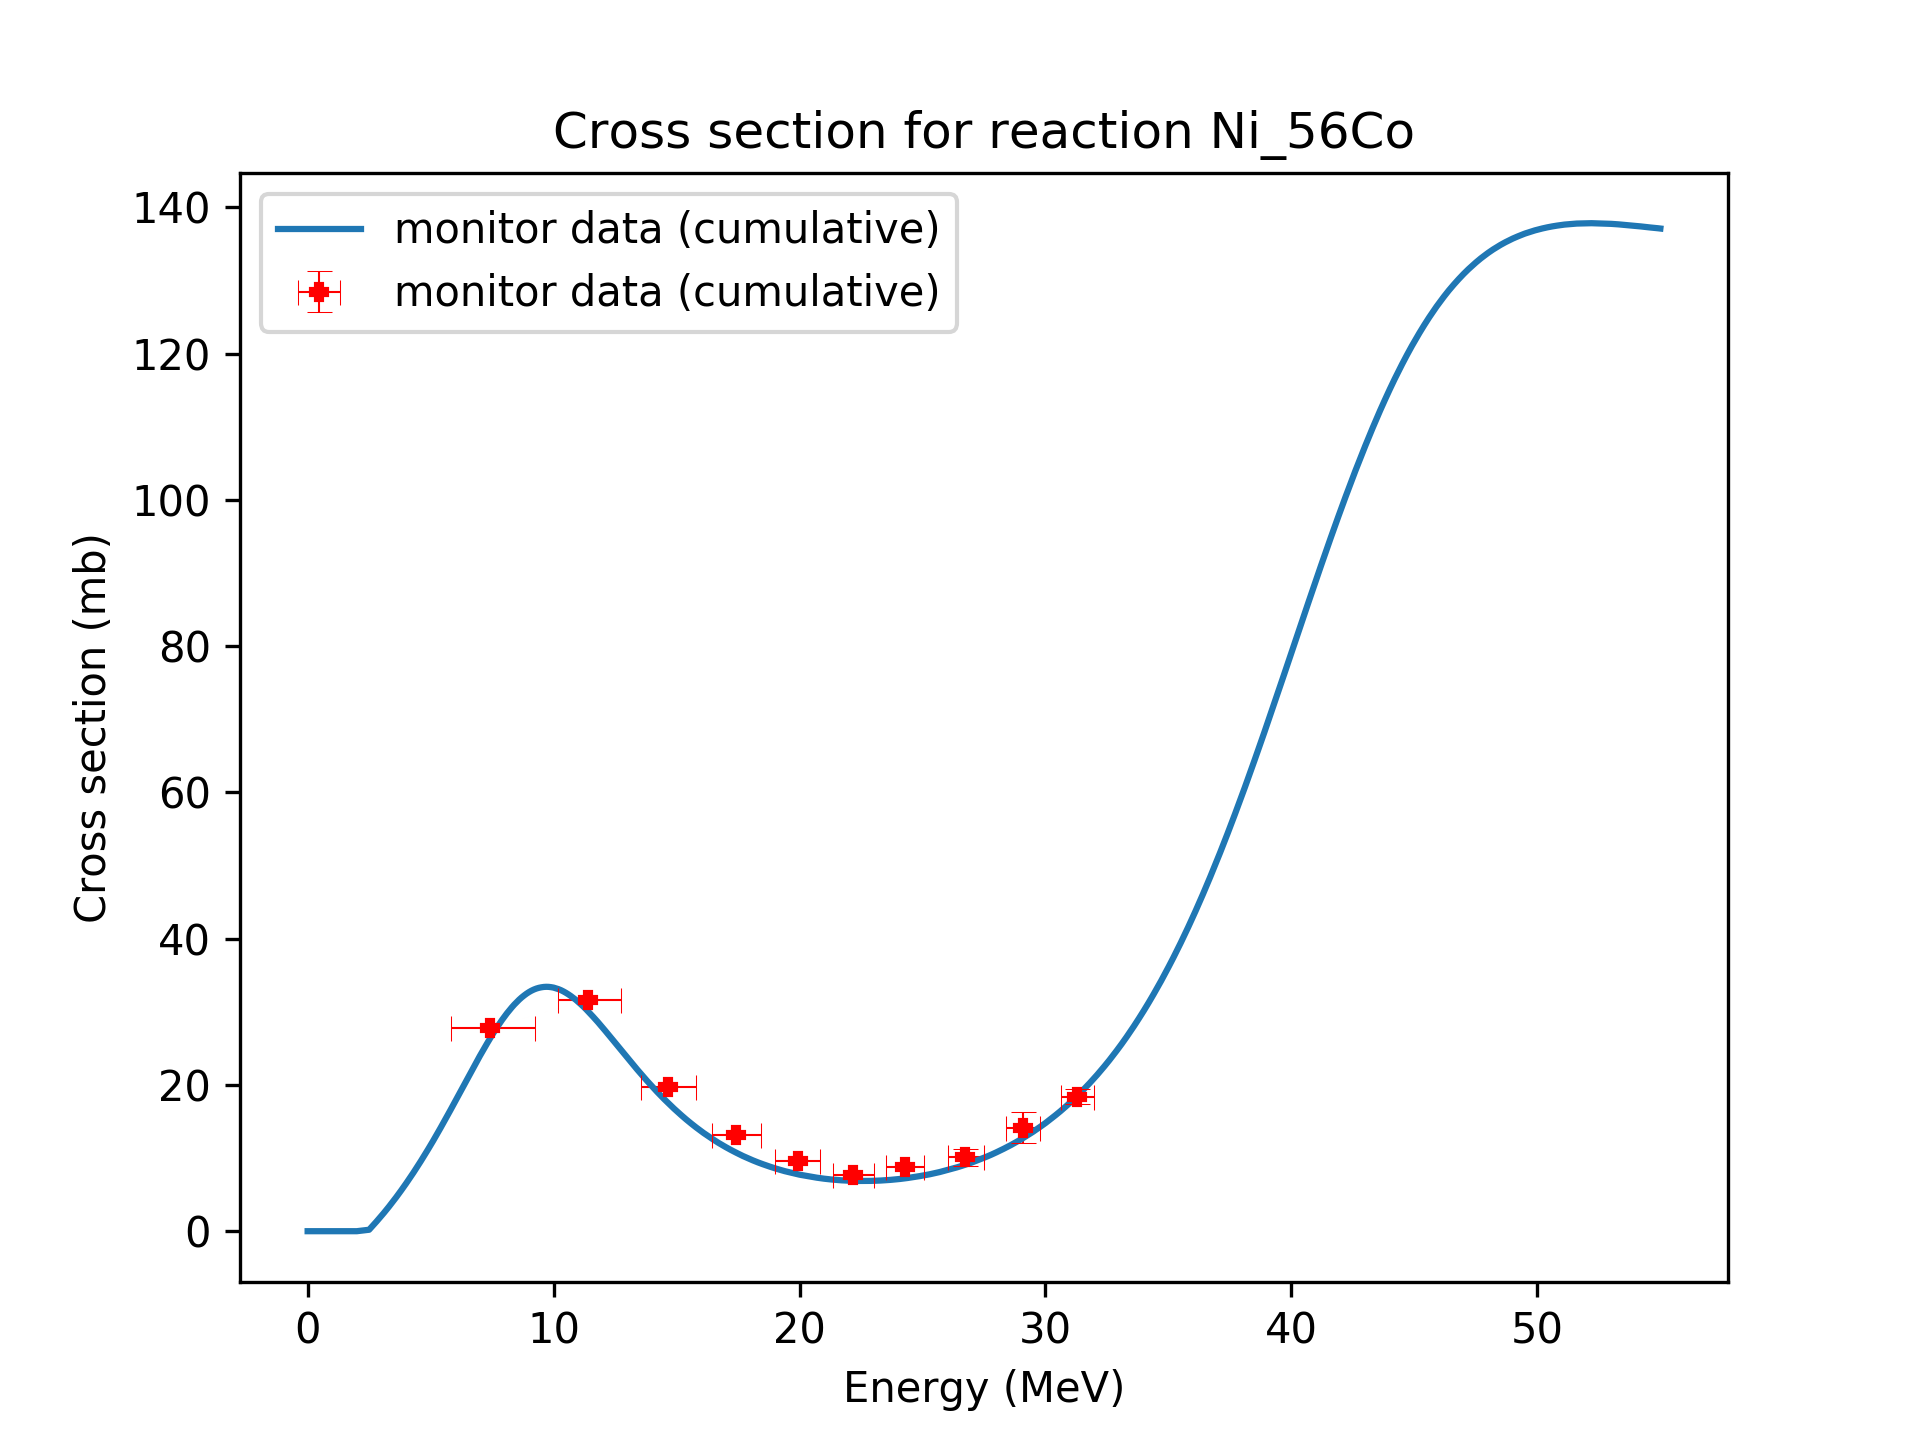
\includegraphics[width=5cm]{Ni_56Co.png} }}%
    \quad
    \subfloat[]{{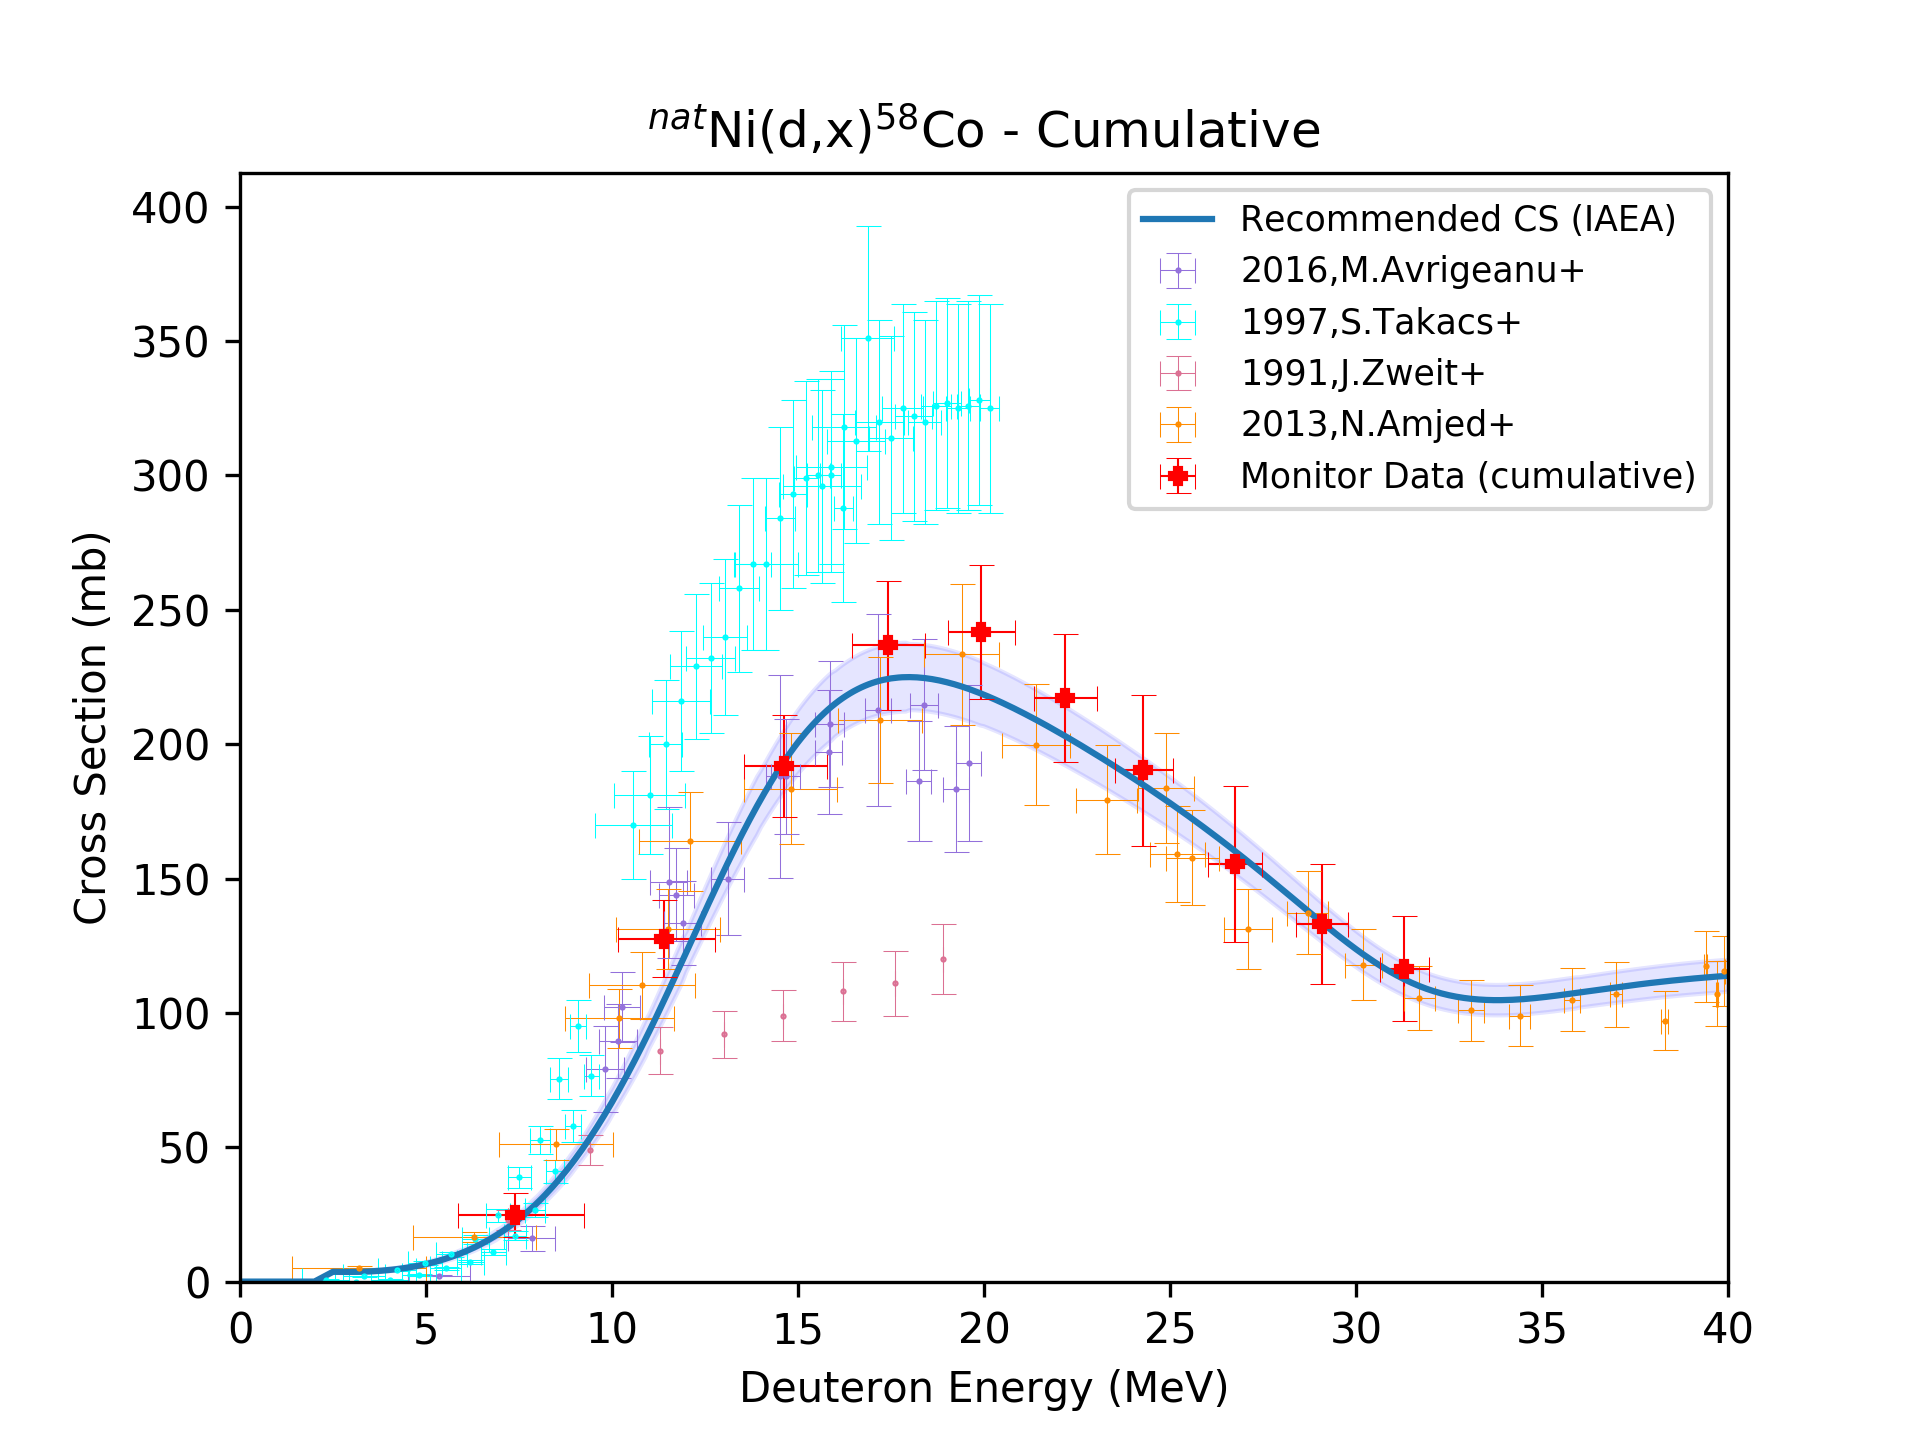
\includegraphics[width=5cm]{Ni_58Co.png} }}%
    \quad
    \subfloat[caption]{{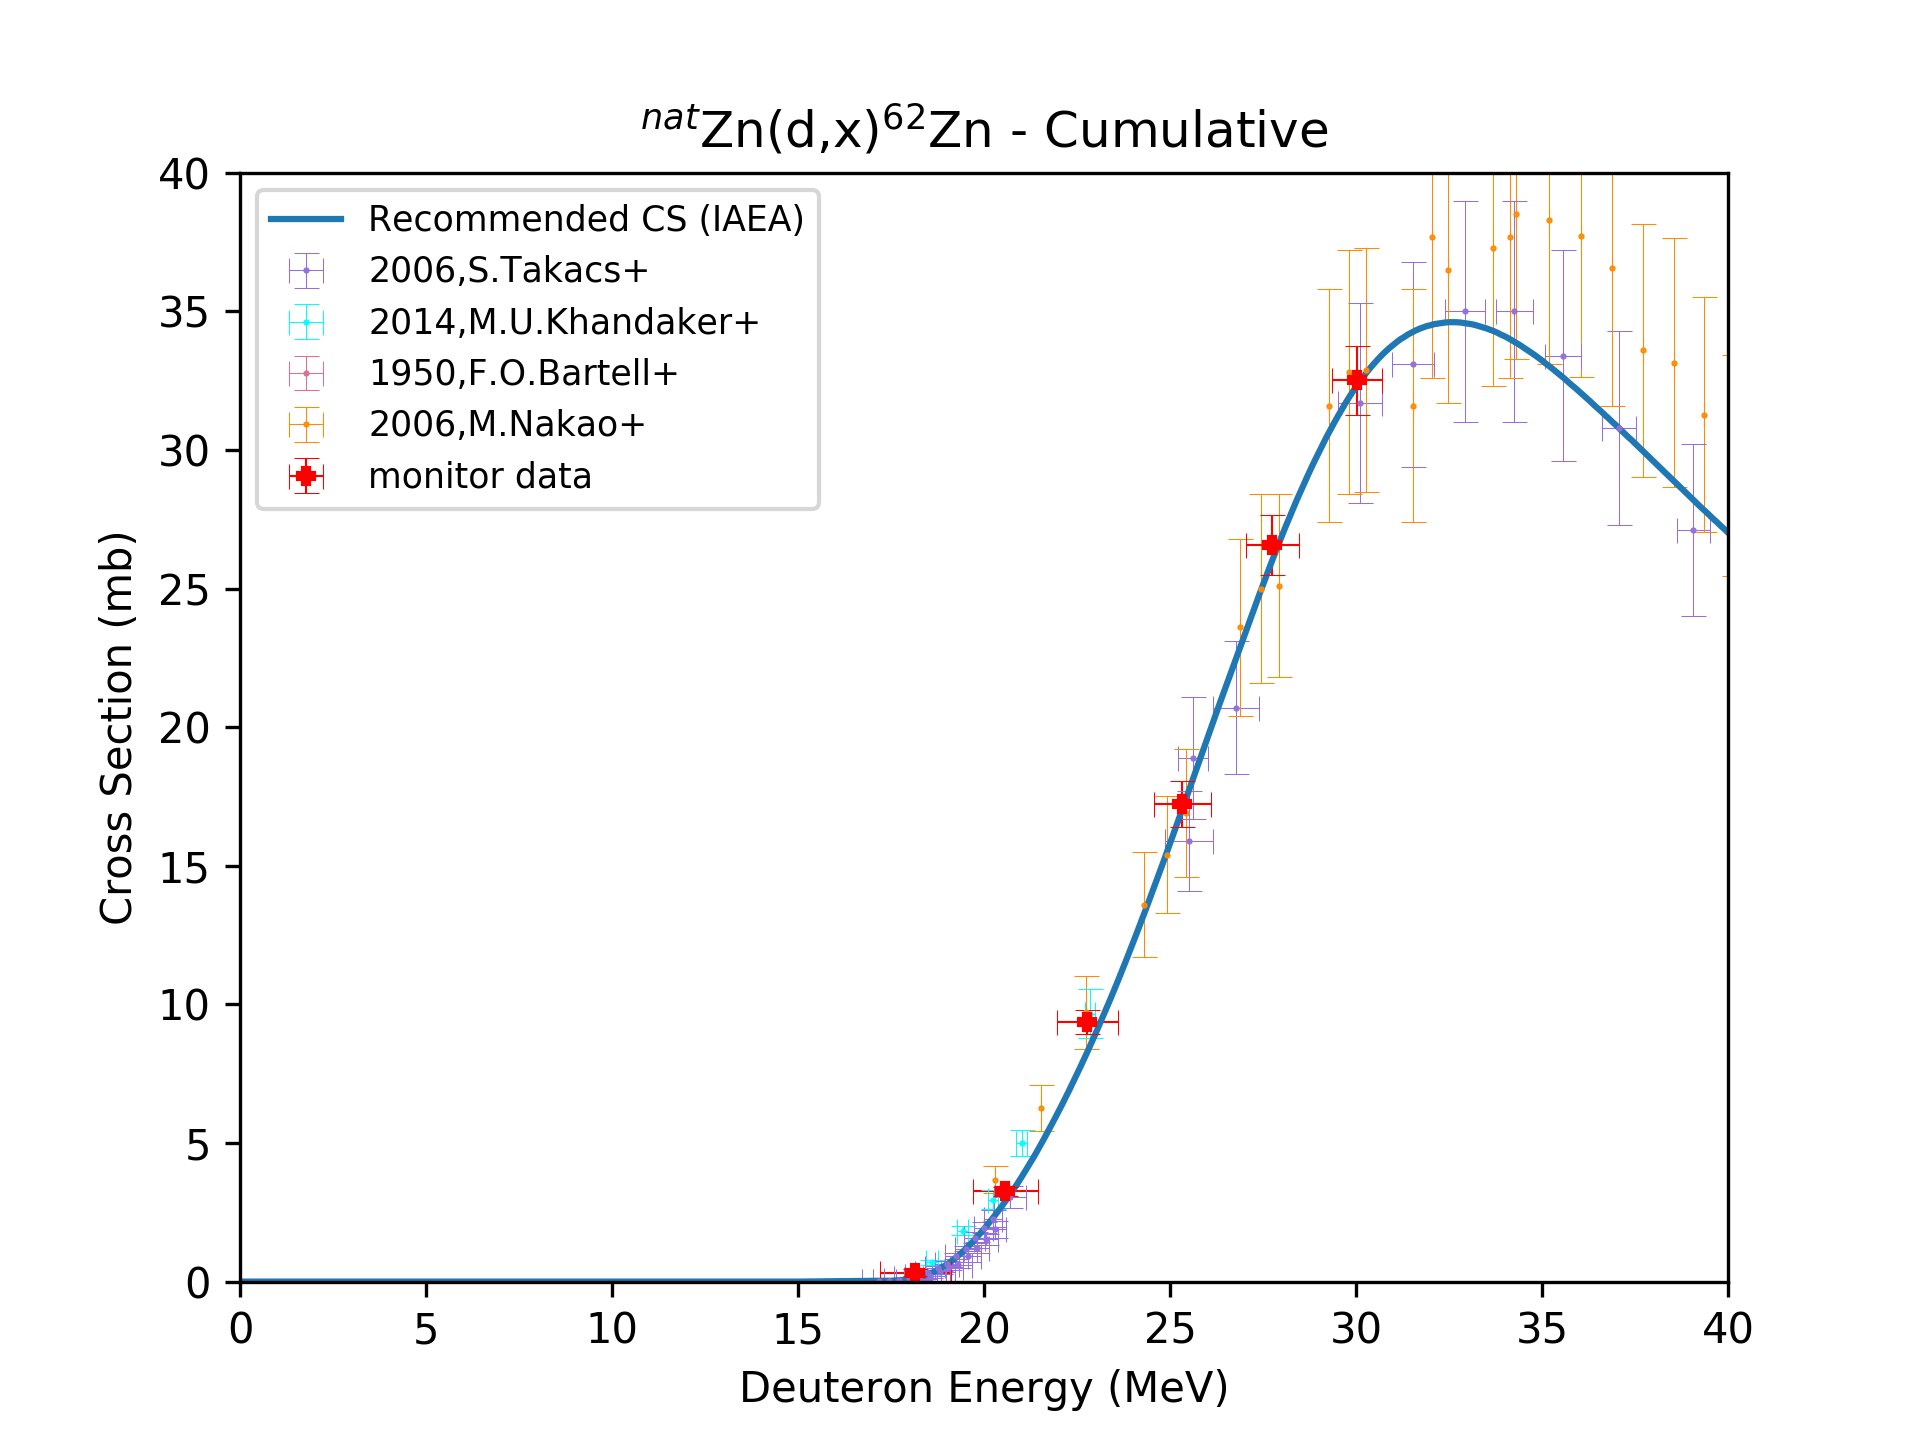
\includegraphics[width=5cm]{Cu_62Zn.png} }}%
    \quad
    \subfloat[]{{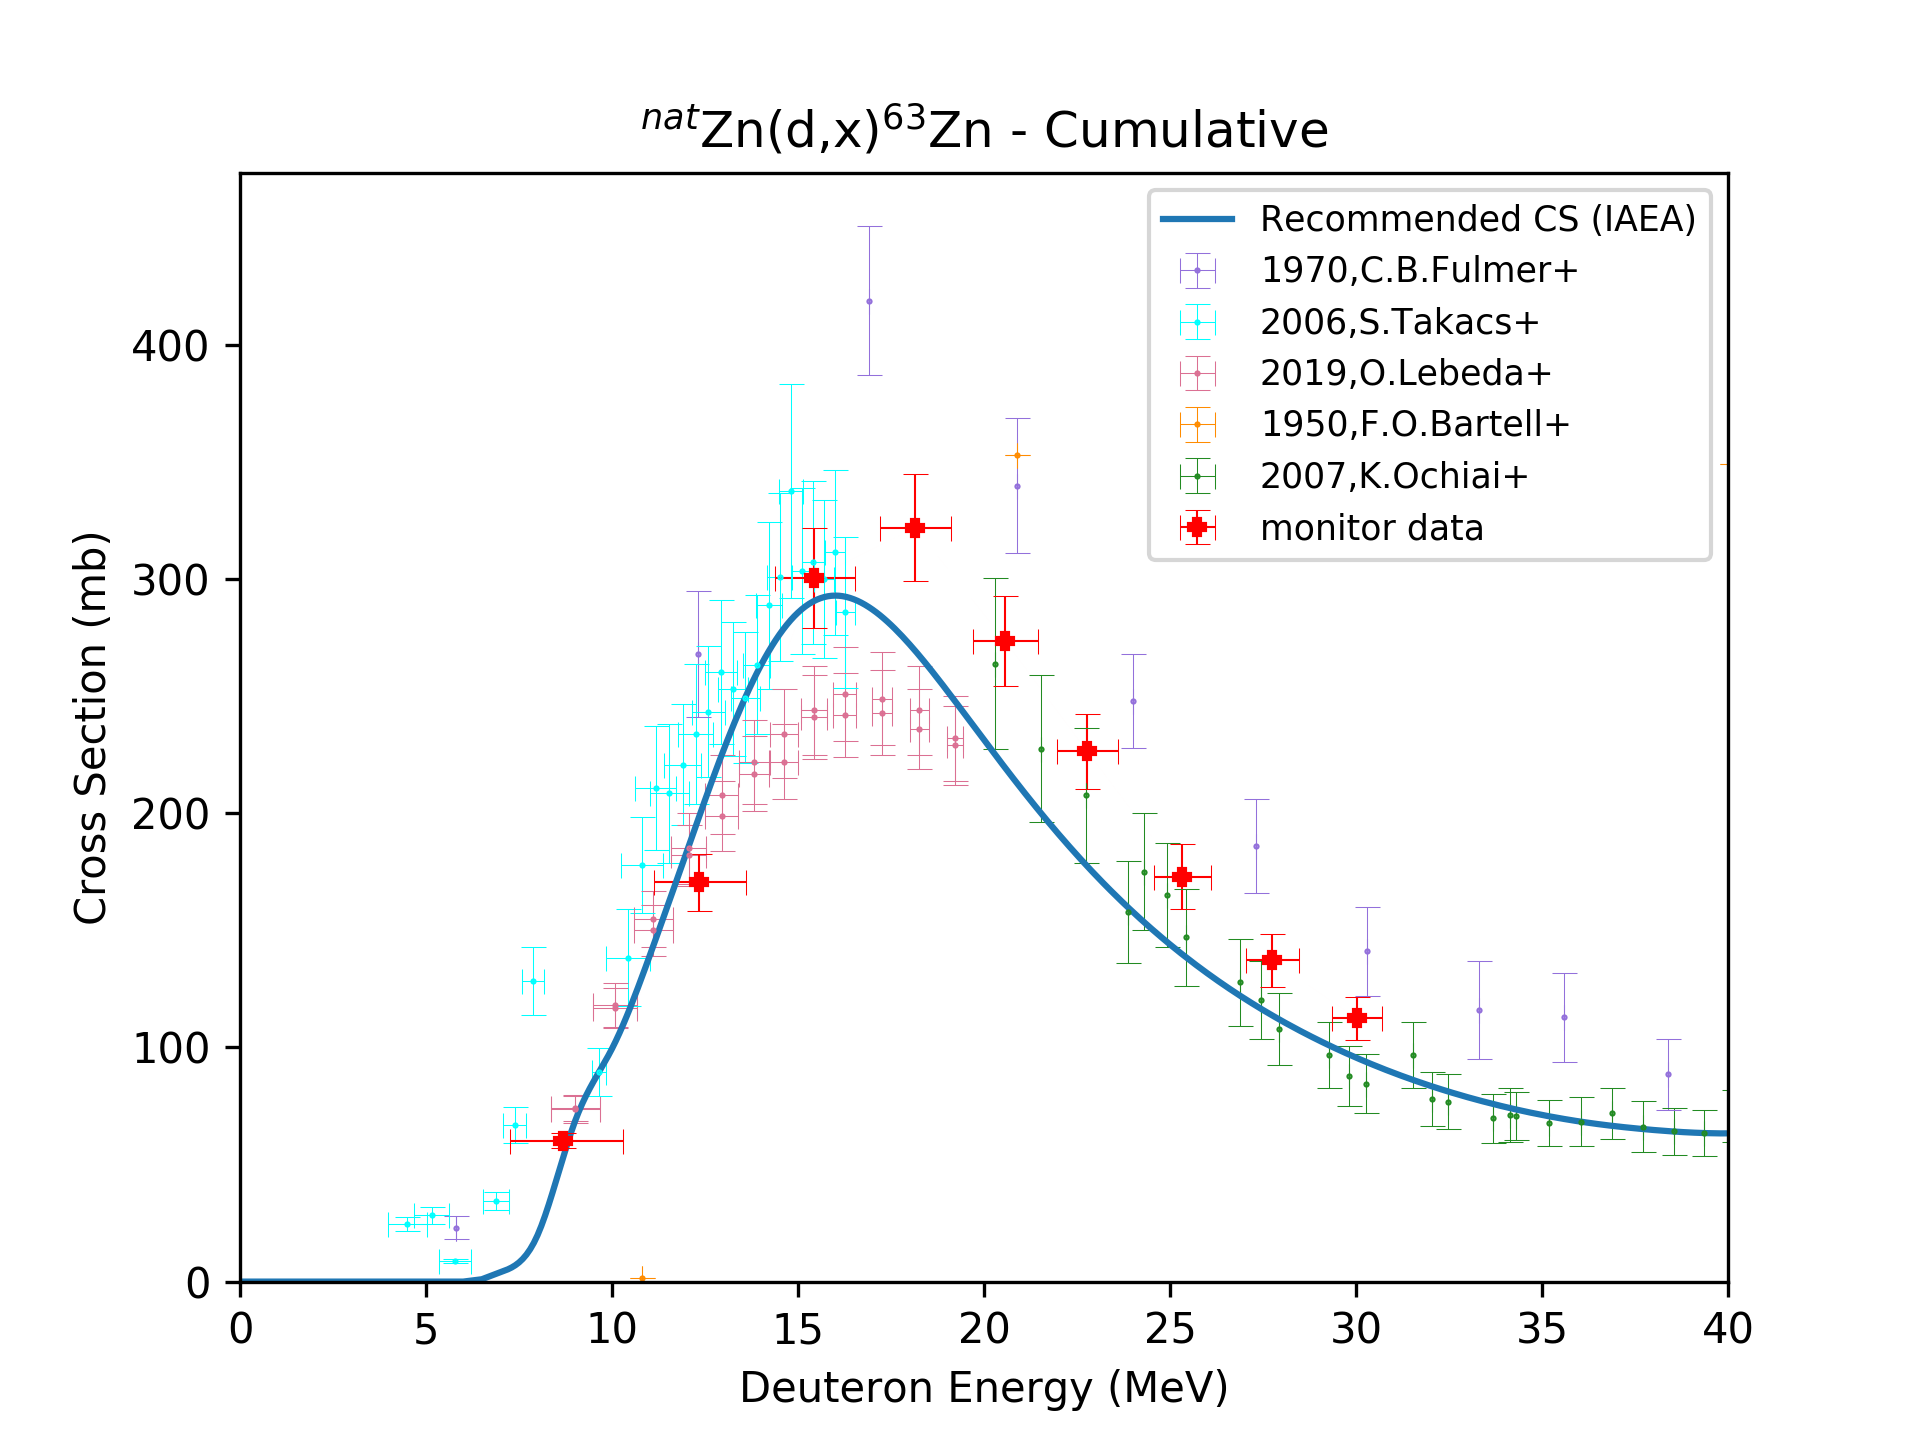
\includegraphics[width=5cm]{Cu_63Zn.png} }}%
    \quad
    \subfloat[]{{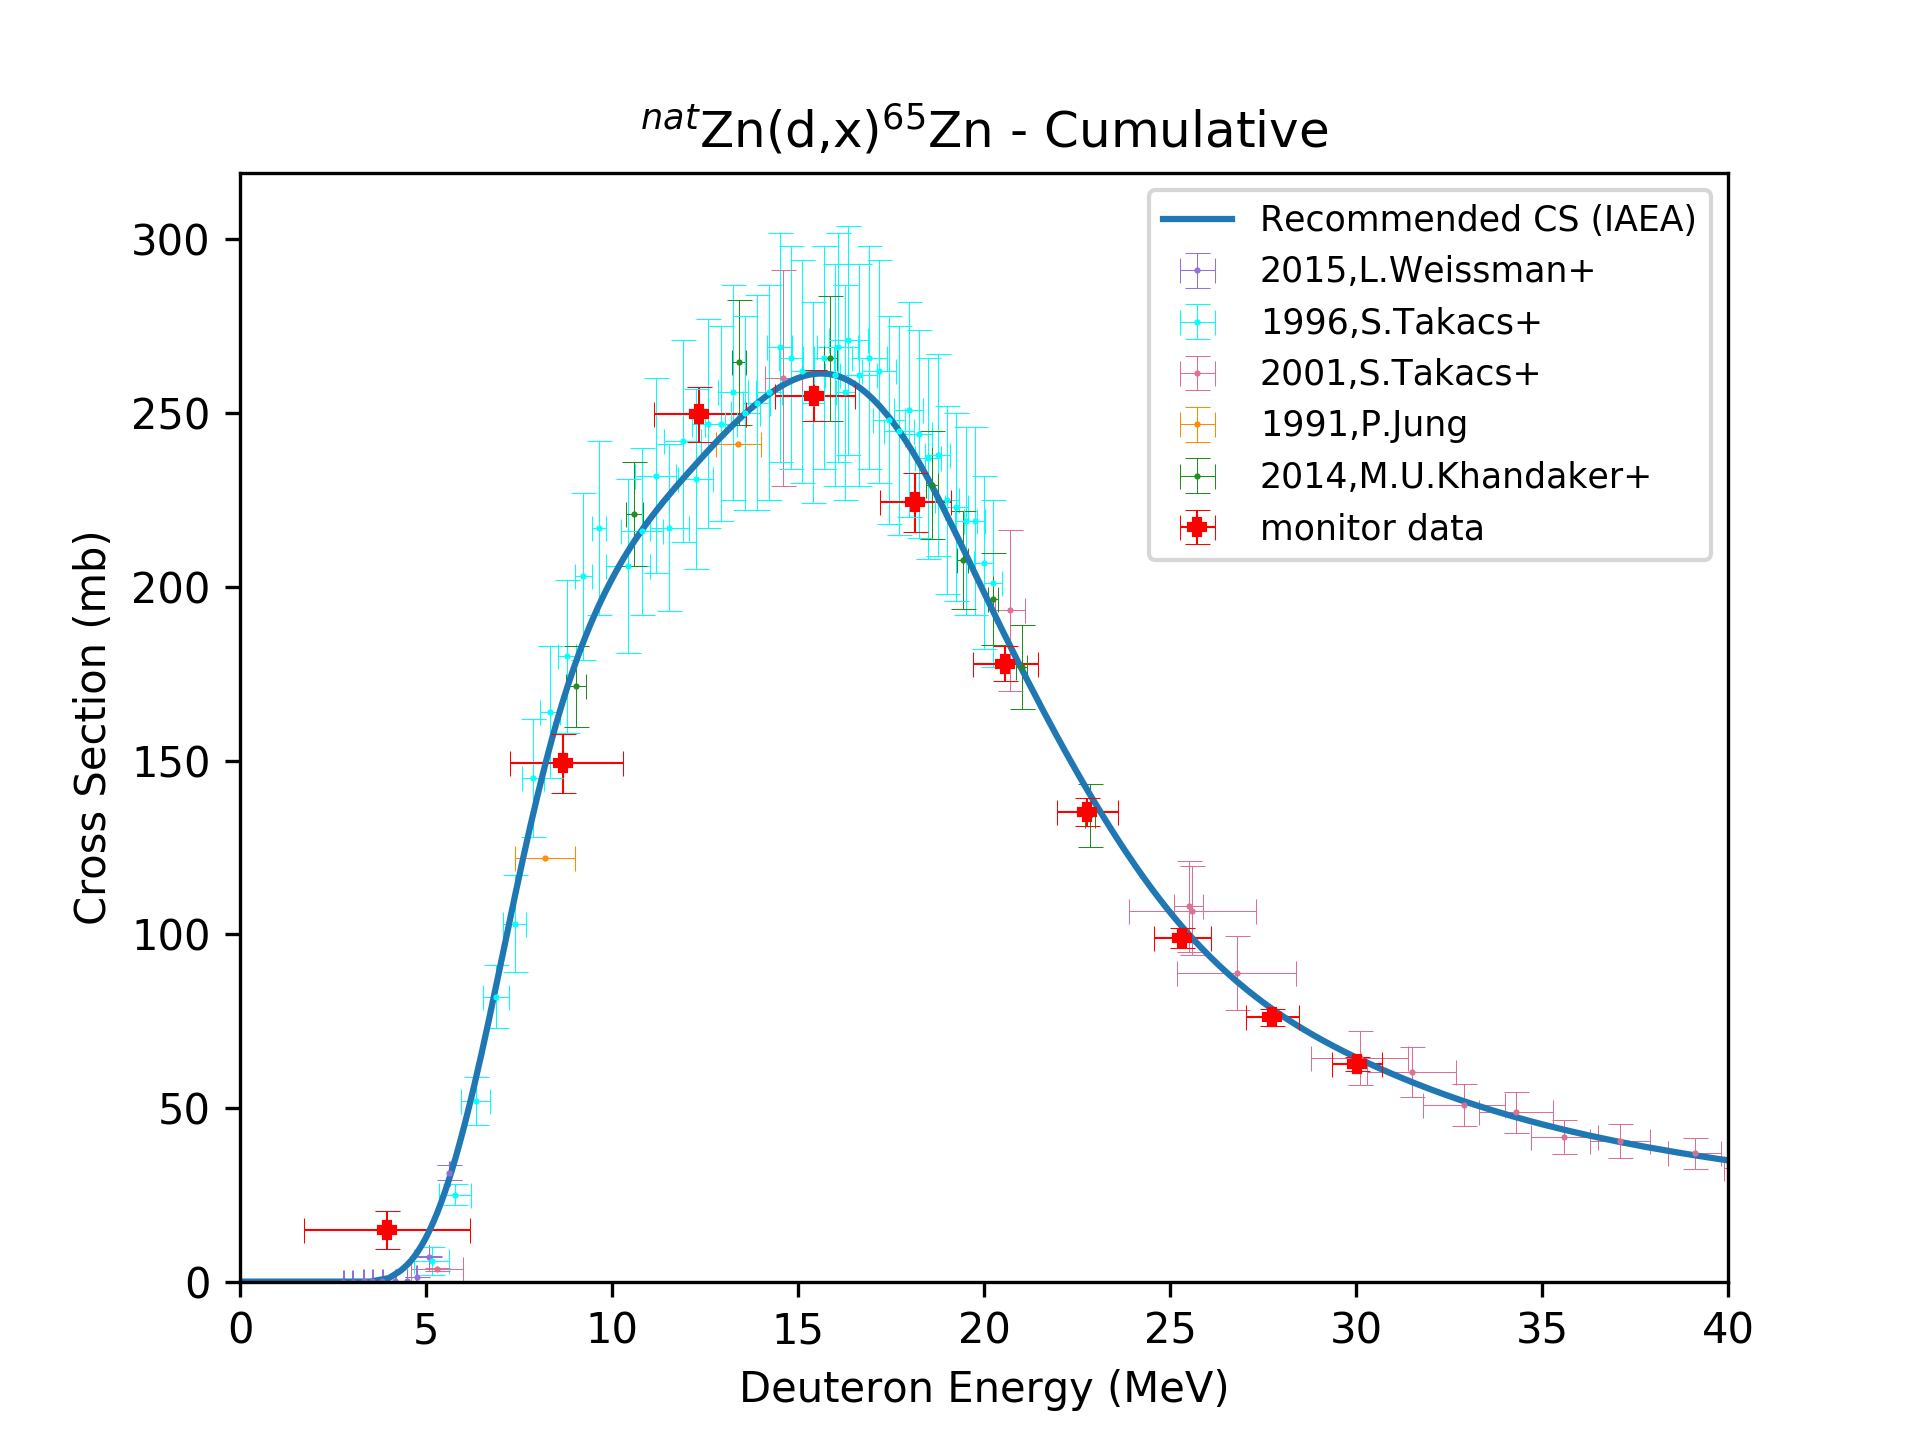
\includegraphics[width=5cm]{Cu_65Zn.png} }}%
    \quad
    \caption{Figure shows the estimation of monitor cross section using the calculated beam current. It is compared along with the monitor data.  }%
    \label{fig:monitor_BC}%
\end{figure}



\subsection{Production Cross sections}

Once the weighted average beam current was estimated, the cross sections were estimated using equation \ref{eq:CS_ch3}. For decay chains, the first observed element was reported as cumulative, unless it was the first entry. If there was independent measurements of the daughter products, they were reported as independent and cumulative along with the parent. 






